\documentclass[../main.tex]{subfiles}


\begin{document}
En esta sección se exponen los fundamentos del Impresionismo pictórico y de la Inteligencia Artificial, para posteriormente centrarnos en las Redes Neuronales Artificiales y sus modernos sistemas con el objetivo de que el lector comprenda las técnicas utilizadas en este \tfg. Para ampliar conocimientos, remitimos a la bibliografía que citaremos a lo largo de este Capítulo.

\section{Impresionismo Pictórico}
Como ya comentamos brevemente en la introducción, el Impresionismo pictórico es un estilo originado en Francia en la segunda mitad del siglo XIX, que se caracteriza por su persistente experimentación con la iluminación \cite{Todocuadros}, ya que se considera como un factor crucial para generar belleza.

\subsection{Origen del nombre}

En abril de 1874 se organiza la primera exhibición de un grupo de jóvenes pintores franceses, cansados del enfoque conversador que imperaba en la Académie des Beaux-Arts (Academia de Bellas Artes). Tras la exposición aparecen las primeras reseñas, siendo esta la que daría nombre al movimiento:
\begin{center}
    \begin{minipage}{0.9\linewidth}
        \vspace{5pt}%margen superior de minipage
        {\small
            Impresión, desde luego eso produce. Simplemente me estaba diciendo que, ya que estaba impresionado, tenía que haber alguna impresión en ello … ¡y qué libertad, qué facilidad de fabricación! El papel tapiz en su estado embrionario es más acabado que ese paisaje marino.
        }
        \begin{flushright}
            Louis Leroy, sobre “Impresión, Sol naciente” (figura \ref{fig:monet_amanecer}) \cite{Sienra2019}
        \end{flushright}
        \vspace{3pt}%margen inferior de la minipage
    \end{minipage}
\end{center}

\begin{figure}[h]
    \centering
    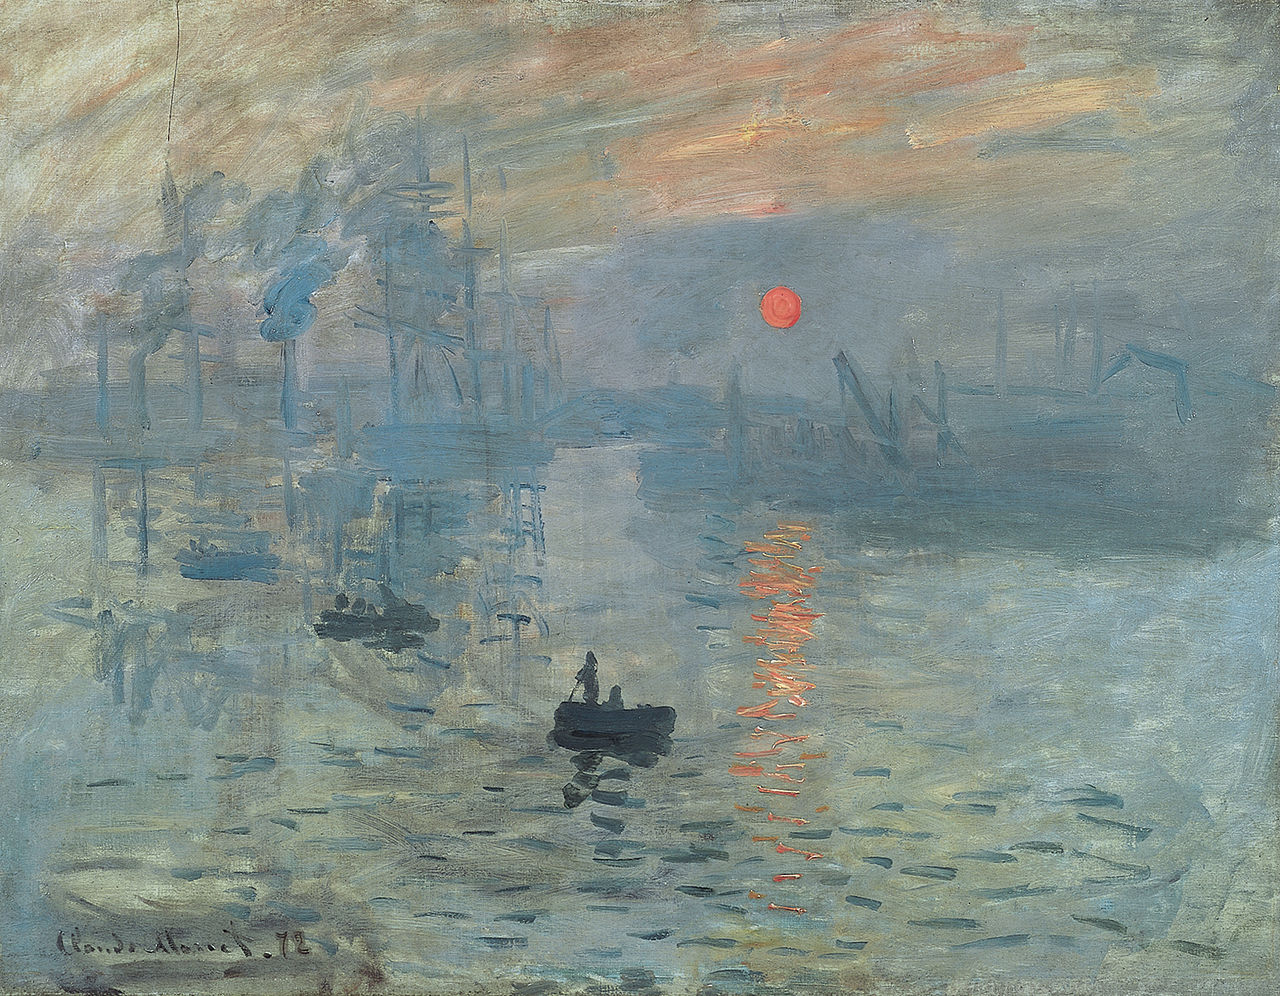
\includegraphics[width=0.45\textwidth]{imagenes/Monet_Amanecer.jpg}
    \caption[Impresión, Amanecer, de Claude Monet]{Impresión, Amanecer, de Claude Monet (Musée Marmontan Monet, Paris). Extraído de \cite{Monet1873}.}
    \label{fig:monet_amanecer}
\end{figure}

Dicha crítica despectiva, en lugar de ridiculizar al movimiento, lo da a a conocer y lo expande rápidamente.

\subsection{Contexto artístico e histórico}

Antes de la aparición del Impresionismo, el estilo predominante en Europa era el Realismo: abandonaron la nostalgia propia del Romanticismo en favor de proyectar los ideales en el porvenir. El hombre pasa a soñar partiendo de la realidad, por lo que el arte se torna \textit{realista} \cite{EditorialSalvat2006}.

\begin{figure}[h!]
    \centering
    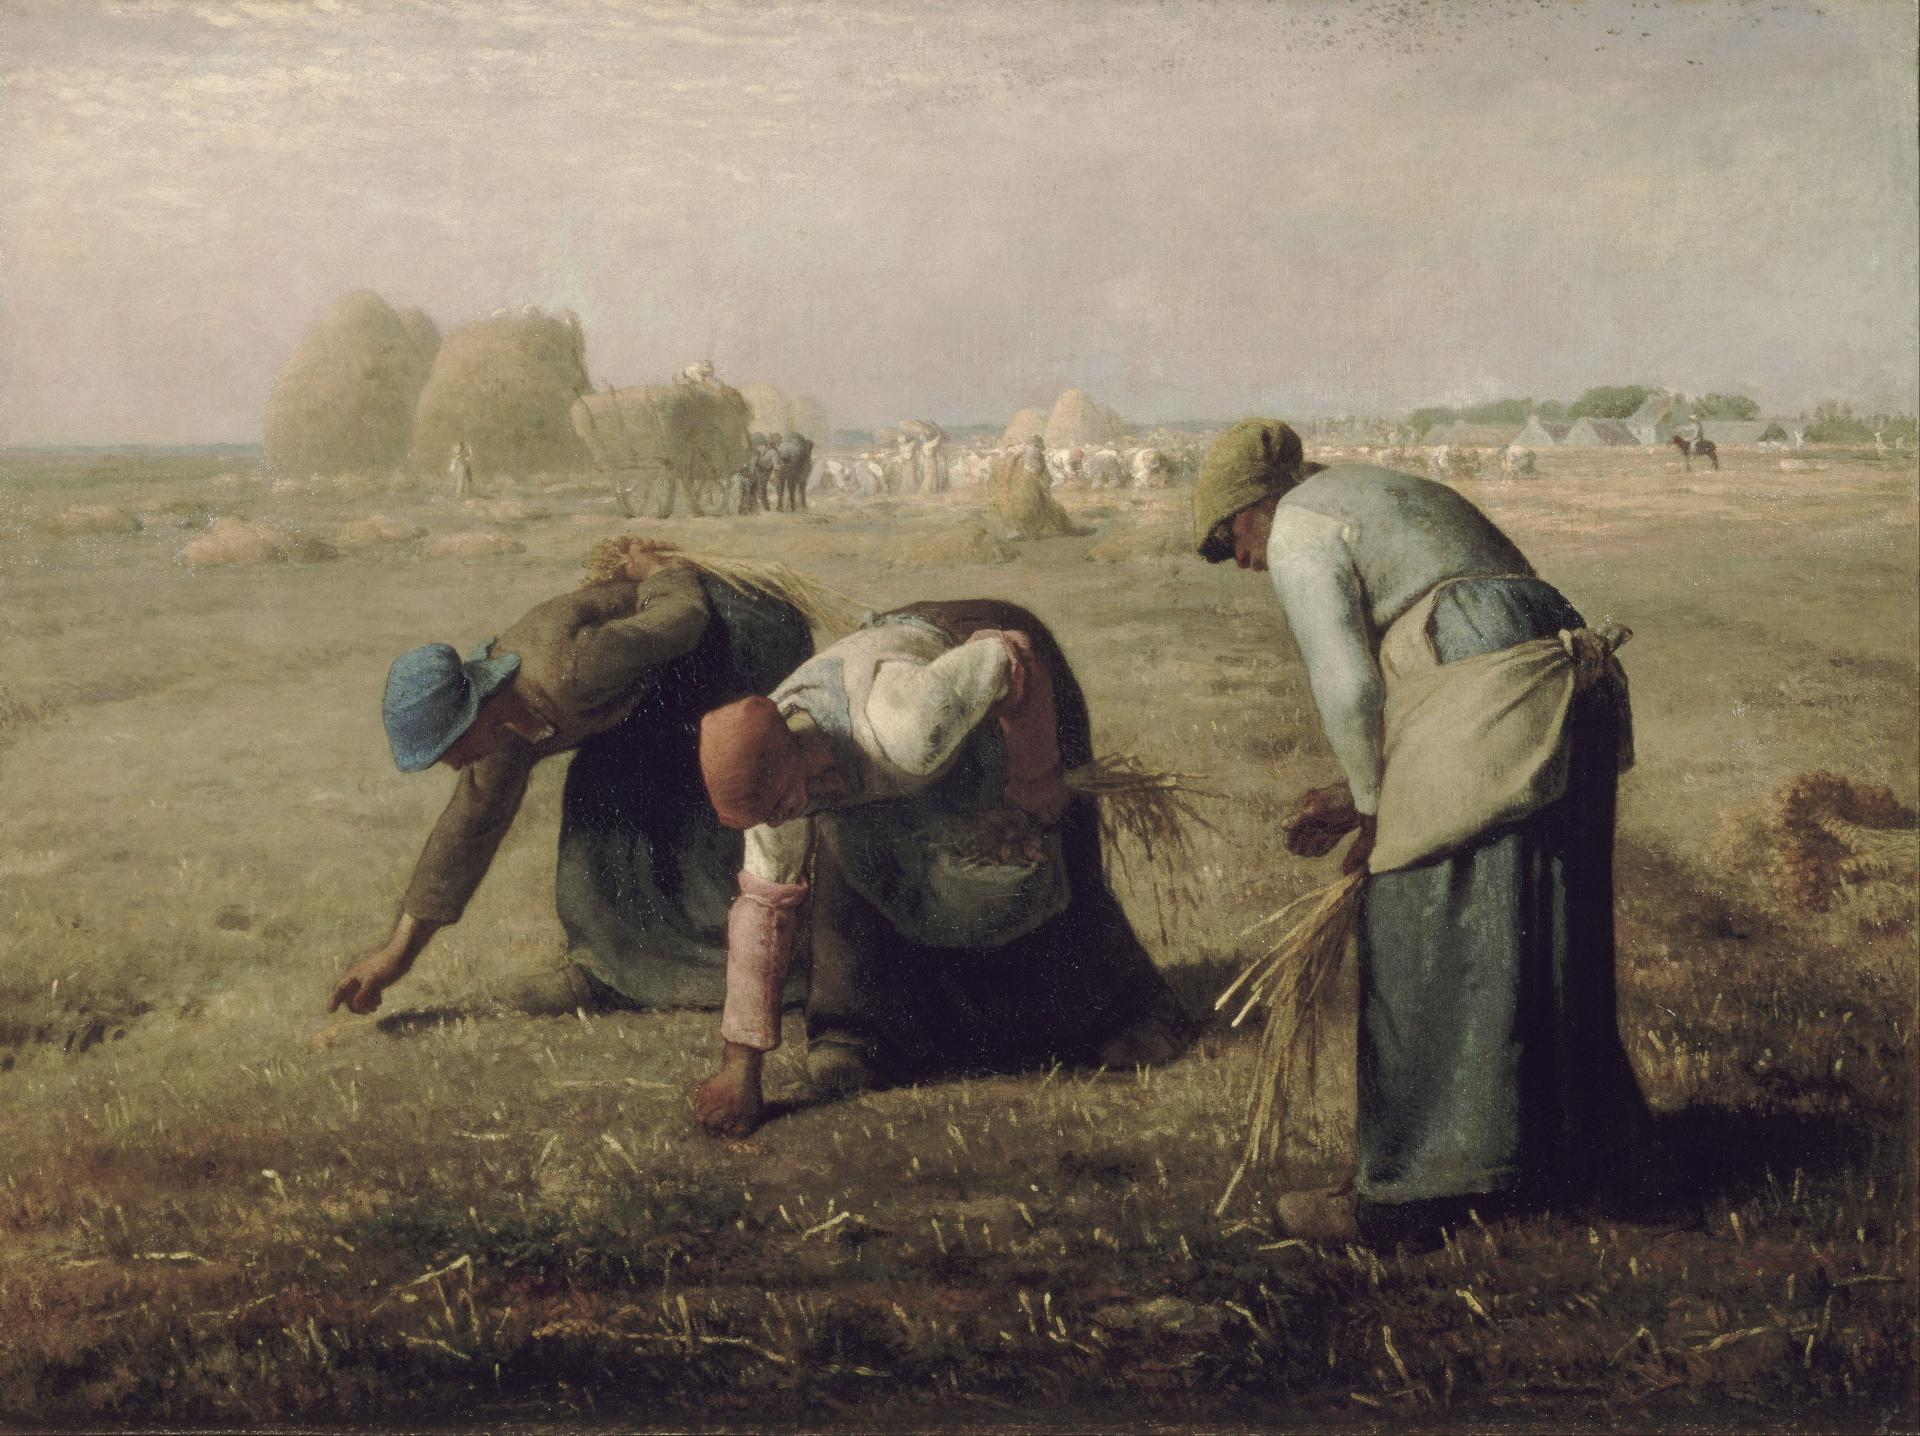
\includegraphics[width=0.5\textwidth]{imagenes/Las espigadoras.jpg}
    \caption[Las espigadoras, de Jean-François Millet]{Las espigadoras, de Jean-François Millet (Musée d'Orsay). Año 1857. Extraído de \cite{Millet1857}.}
    \label{fig:millet_espigadoras}
\end{figure}

Entre finales del siglo XVIII y la primera mitad del siglo XIX el mundo sufre una enorme cantidad de transformaciones: la segunda revolución industrial, las revolución francesa, la Europa de la Restauración Absolutista y las reformas burguesas. La sociedad entra en ebullición a todos los niveles, apareciendo corrientes filosóficas como el Positivismo y el Socialismo, mientras se publican obras tan influyentes como el Manifiesto Comunista de Karl Marx (1848).
\newline

En mitad de esta vorágine, los impresionistas reaccionan dando un mayor peso a la luz y el color; aspectos que toman de la pintura veneciana de mediados del siglo XVI y de la pintura holandesa del siglo XVII.

\begin{figure}[h!]
    \centering
    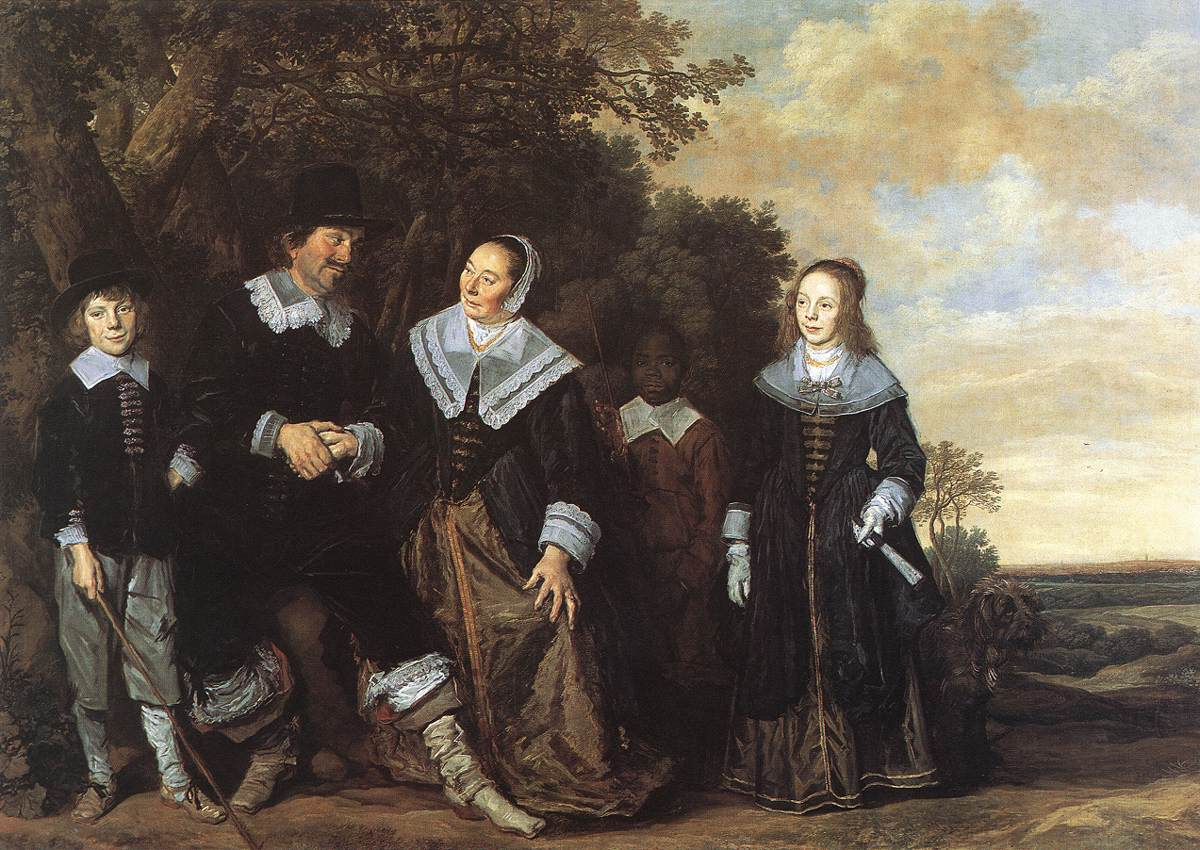
\includegraphics[width=0.5\textwidth]{imagenes/Grupo familiar ante un paisaje.jpg}
    \caption[Grupo familiar ante un paisaje, de Frans Hals]{Grupo familiar ante un paisaje, de Frans Hals (Museo Nacional Thyssen-Bornemisza). Pintura holandesa del año 1648. Extraído de \cite{Hals1648}.}
    \label{fig:hals_familia}
\end{figure}

\subsection{Características artísticas}

El Impresionismo se revela como una contestación al Realismo, ya que donde el Realismo presenta determinación, el Impresionismo muestra "lo continuo e indefinido, por la inestabilidad y el cambio perpetuo, incapaz de ofrecer una visión precisa de la realidad. De ahí las formas imprecisas, el toque distendido, la incertidumbre total" \cite{EditorialSalvat2006}. Ese cambio de filosofía se expresa con los siguientes rasgos \cite{Sienra2019}:
\begin{itemize}
    \item La importancia de la luz: como ya hemos mencionado anteriormente, muchos autores practicaban la pintura al aire libre, por lo que pudieron estudiar de cerca la luz y sus efectos en la naturaleza.
    \item Pinceladas gruesas y pictóricas: los impresionistas emplean pinceladas gruesas, como si se tratase de un boceto. Esto permite capturar la naturaleza efímera y fugaz a la vez que experimentaban con el color y las formas que interactúan sobre el lienzo. Observe la figura \ref{fig:cezanne_sena}.
    
    \begin{figure}[h]
        \centering
        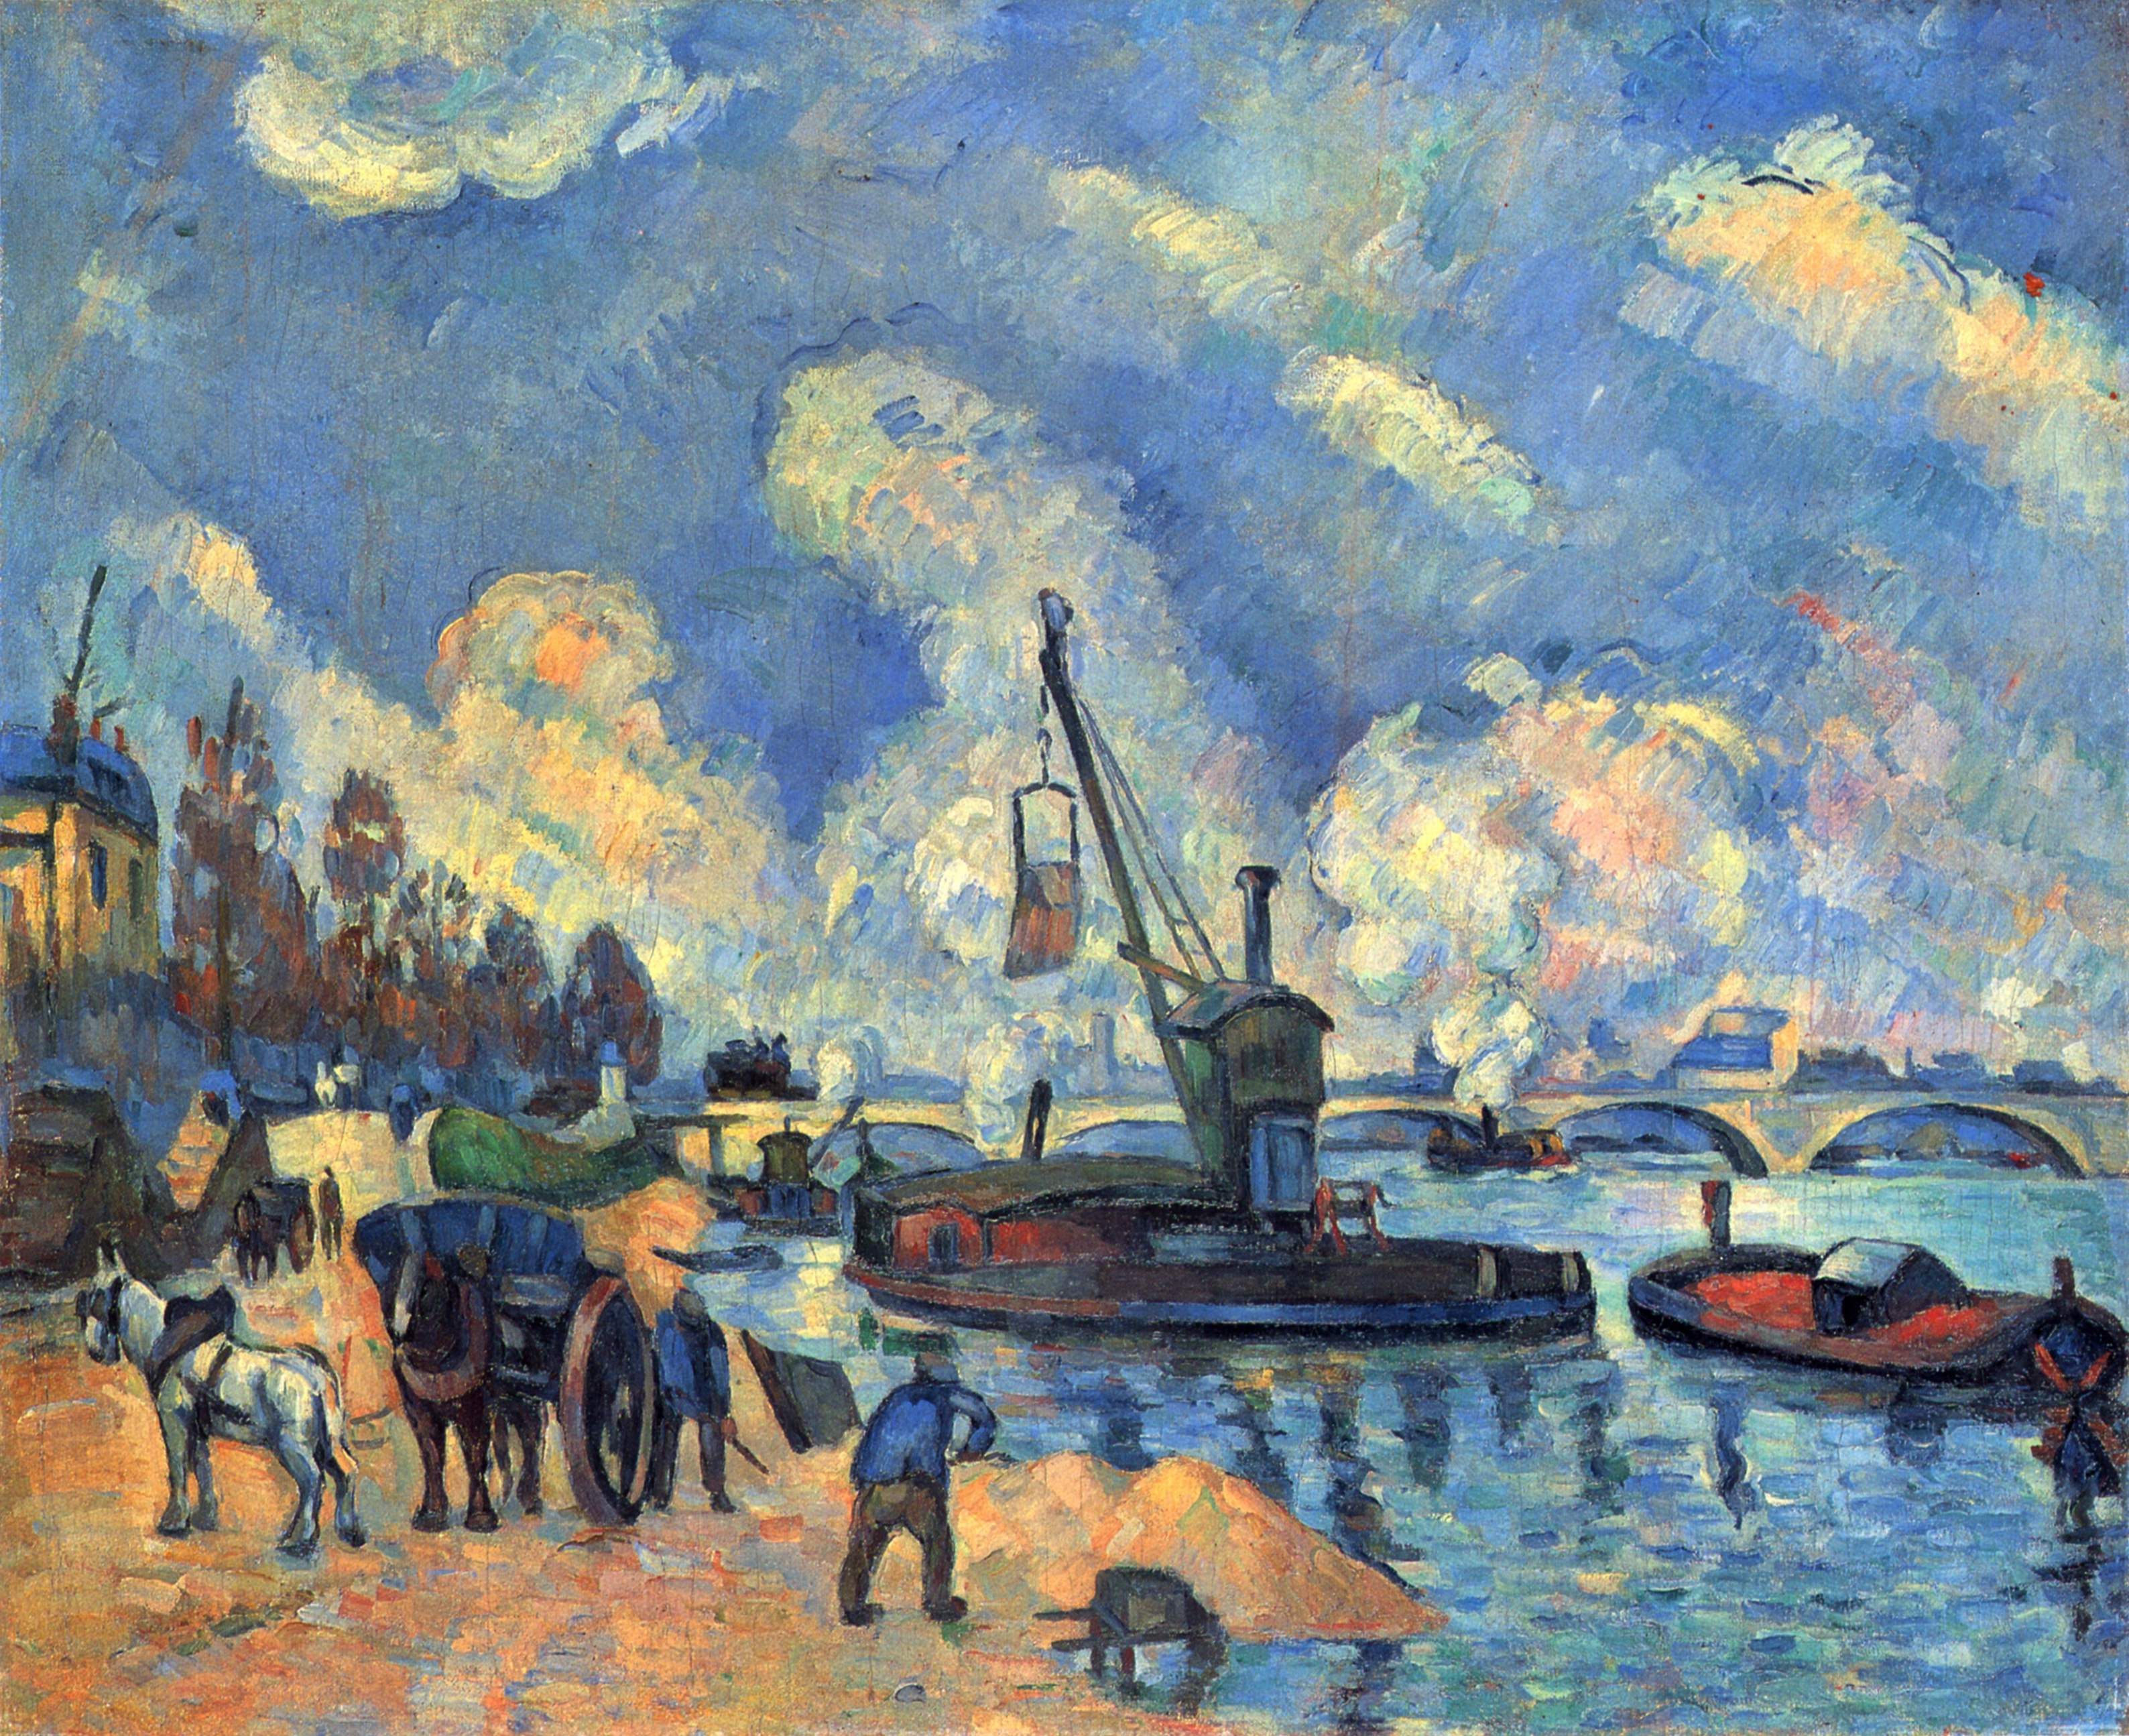
\includegraphics[width=0.6\textwidth]{imagenes/El Sena en Bercy.jpg}
        \caption[El Sena en Bercy, de Paul Cézanne]{El Sena en Bercy, de Paul Cézanne. Extraído de \cite{Cezanne1878}.}
        \label{fig:cezanne_sena}
    \end{figure}
    
    \item Una distintiva paleta de colores: en lugar de mezclar la pintura para obtener nuevos tonos, agrupaban pinceladas individuales de varios colores. Este método se puede observar en las representaciones de sombras y nieves, que nunca son completamente negras o blancas, respectivamente. También suelen presentar esquemas de colores neutros con toques vivos de rojo que atraen la vista y dan equilibrio a las composiciones. Puede apreciarse esta nueva paleta en la figura \ref{fig:monet_terraza}.
    \begin{figure}[h]
        \centering
        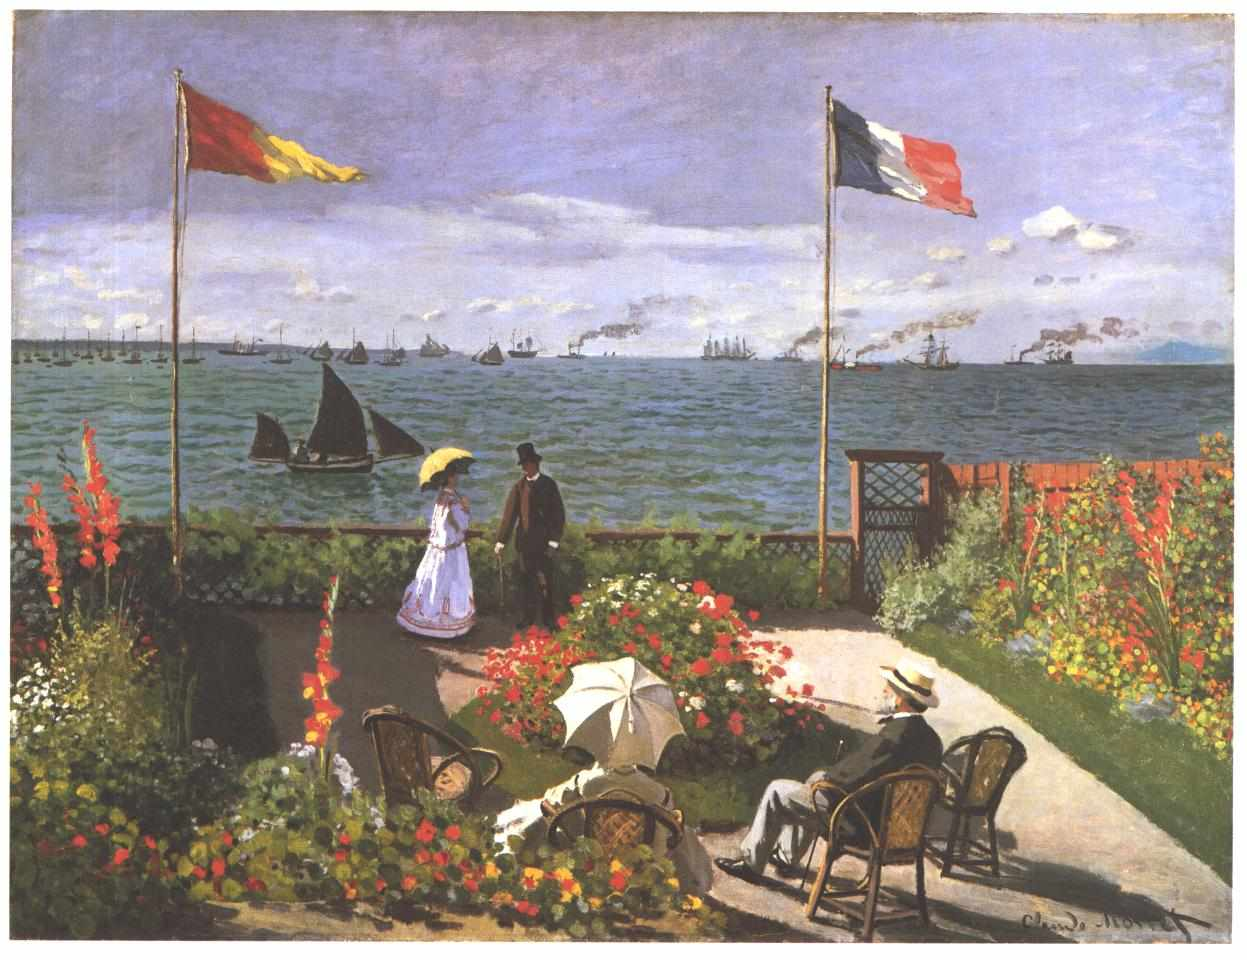
\includegraphics[width=0.66\textwidth]{imagenes/La terraza de Sainte-Adresse.jpg}
        \caption[La terraza de Sainte-Adresse, de Claude Monet]{La terraza de Sainte-Adresse, de Claude Monet (Metropolitan Museum of Art, Nueva York). Año 1867. Extraído de \cite{Monet1867}.}
        \label{fig:monet_terraza}
    \end{figure}
    
    \item Sujetos y temas cotidianos: influenciados por el costumbrismo español abanderado por Francisco de Goya, el contenido típico de las pinturas impresionistas incluye bodegones, paisajes, retratos, y escenas urbanas; nada que ver con las escenas históricas, mitológicas y alegóricas de la pintura francesa tradicional.

\end{itemize}

\subsection{Monet}

Claude Monet (1840-1926), pintor francés, fue la figura clave del movimiento expresionista. Dibujante de caricaturas desde niño, ya pintaba paisajes y marinas, algo que le agradaba al poder trabajar al aire libre \cite{CalvoSantos2016}. Su exilio a Argelia para evitar el servicio militar (si bien su familia pagó el reemplazo un año después y pudo regresar a Francia) y sus viajes por Europa hacen que se enamore de las distintas luces intríscecas a los momentos del día. 

\begin{figure}[h!]
    \centering
    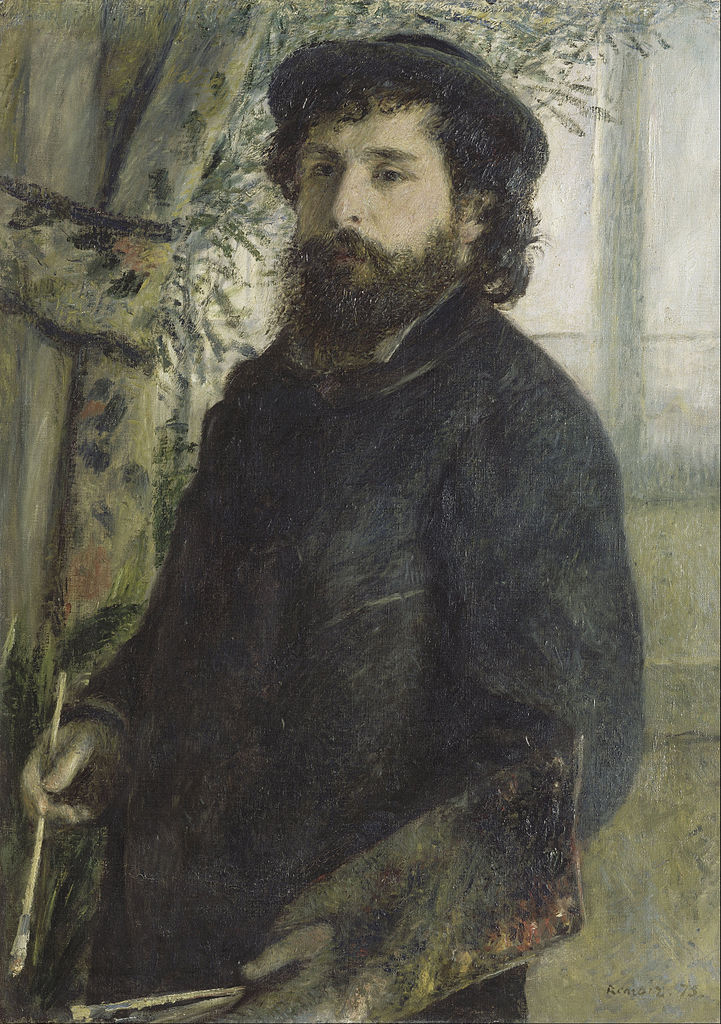
\includegraphics[width=0.4\textwidth]{imagenes/Retrato de Claude Monet.jpg}
    \caption[Retrato de Claude Monet, por Pierre-Auguste Renoir.]{Retrato de Claude Monet, por Pierre-Auguste Renoir (Musée d'Orsay, Paris). Extraído de \cite{Renoir1875}.}
    \label{fig:monet_retrato}
\end{figure}

Sus innovaciones en el estudia de la luz y del color causaron reacciones mixtas, si bien se adelantó lo justo a su tiempo para ser considerado innovador y tener éxito en vida (a diferencia de muchos otros pintores) al mismo tiempo. \newline

\begin{figure}[h!]
    \centering
    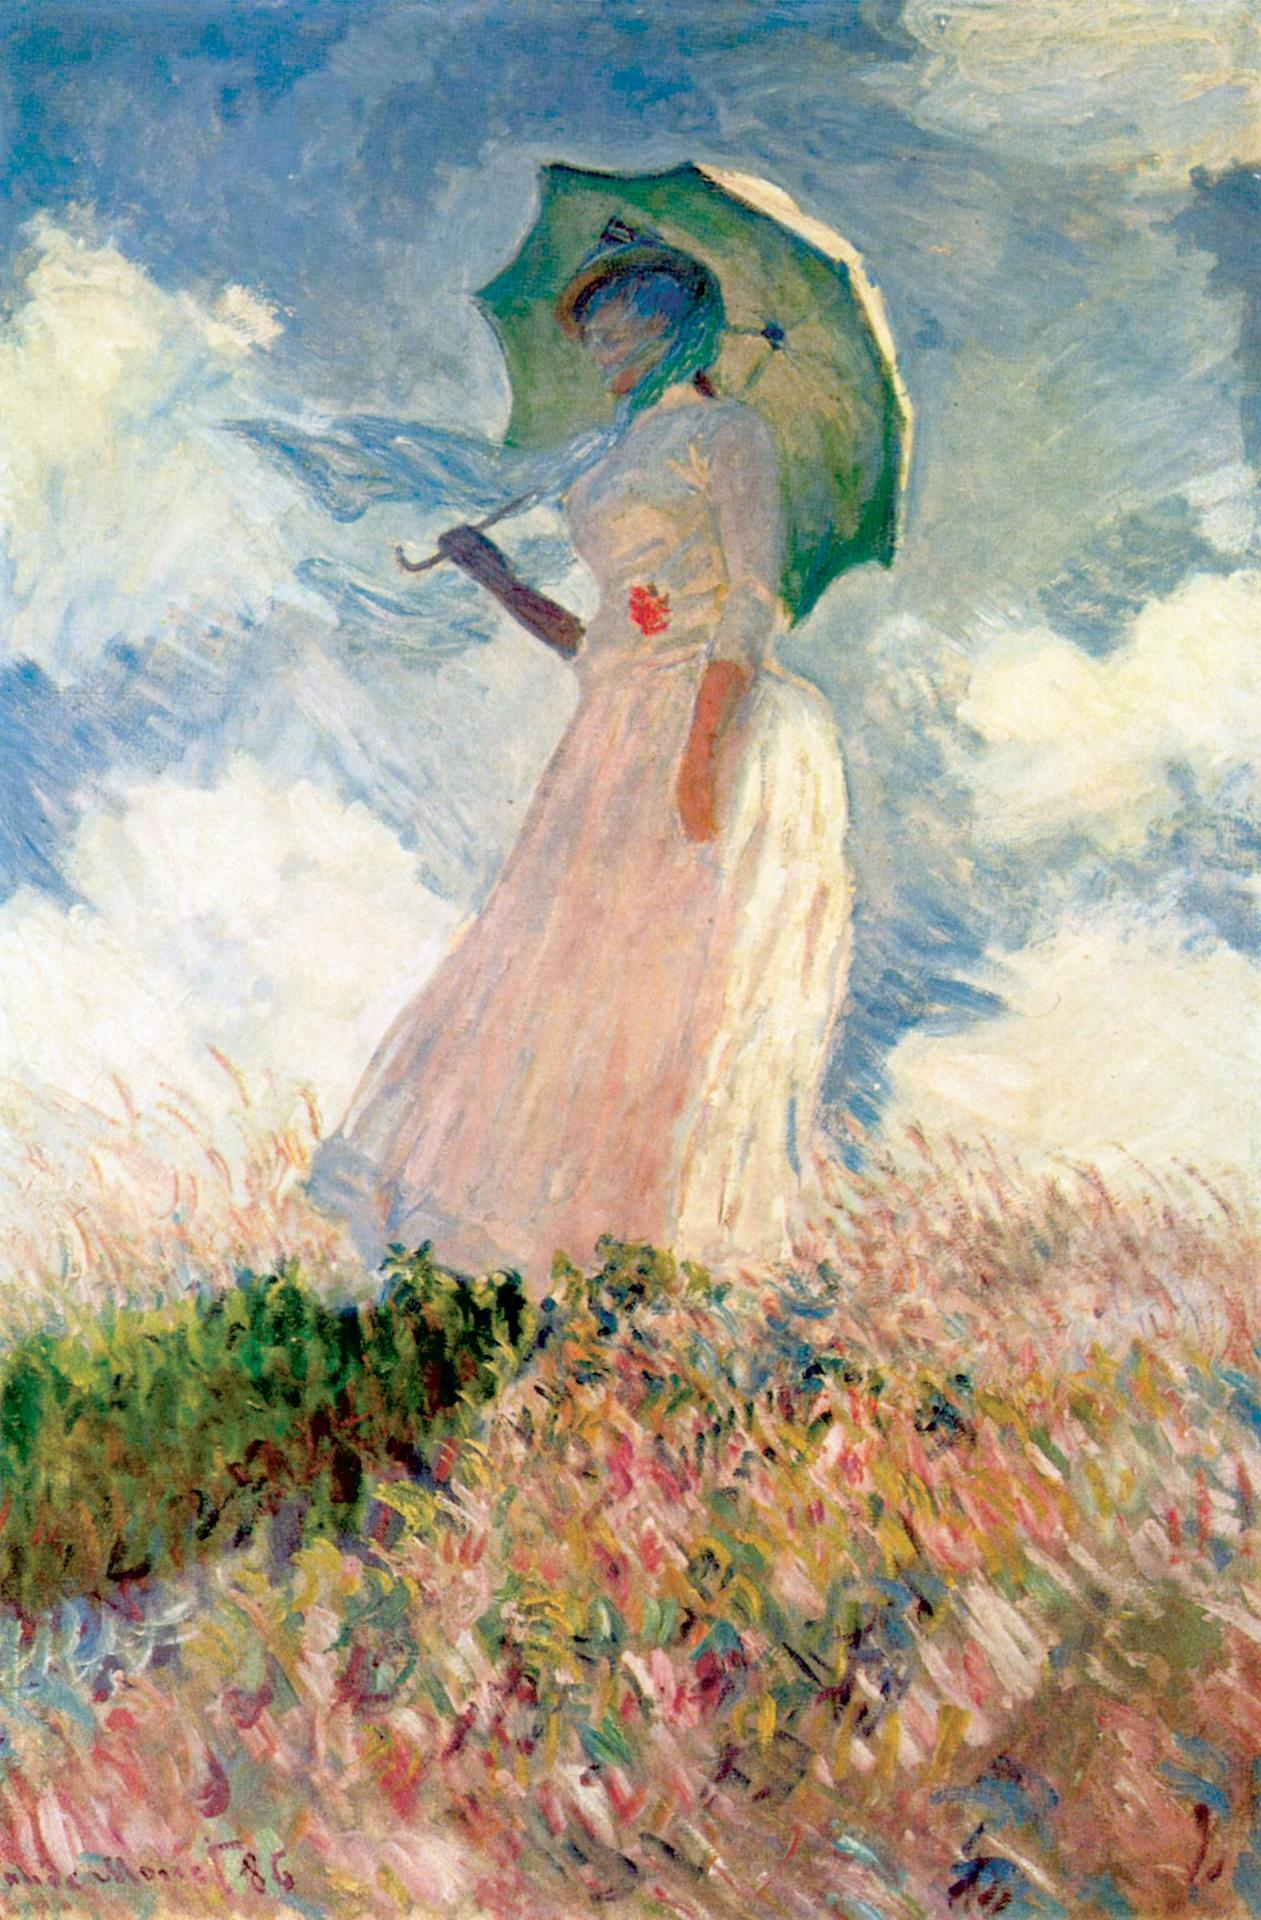
\includegraphics[width=0.4\textwidth]{imagenes/Mujer con sombrilla mirando a la izquierda.jpg}
    \caption[Mujer con sombrilla mirando a la izquierda, de Claude Monet]{Mujer con sombrilla mirando a la izquierda, de Claude Monet (Musée d'Orsay, Paris). Extraído de \cite{Monet1886}.}
    \label{fig:monet_mujer}
\end{figure}

Si bien en sus primeros cuadros tenía un estilo excesivamente experimental y poco comercial, tras la exposición de 1874 en la \textit{Société anonyme des artistes peintres, sculpteurs et graveurs} (Sociedad Anónima de pintores, escultores y grabadores), que cofundó junto a otros pintores, descubrió su estilo: captaba el instante y la luz a través de manchas, lo que junto a su radicalización con el tiempo provocó que en sus últimas obras la forma está ya prácticamente disuelta en manchas de color \cite{CalvoSantos2016}.

Máximo exponente de la pintura en \textit{plein air}, o al aire libre \cite{Sienra2019}, su estilo basado en el cambio del paisaje lo resumió en la siguiente frase.

 \begin{center}
    \begin{minipage}{0.9\linewidth}
        \vspace{5pt}%margen superior de minipage
        {\small
            Para mí, un paisaje no existe por derecho propio, ya que su apariencia cambia en cada momento; pero la atmósfera circundante le da vida –la luz y el aire que varían continuamente. Para mí, es solo la atmósfera circundante la que da a los sujetos su verdadero valor.
        }
        \begin{flushright}
            Claude Monet \cite{Sienra2019}
        \end{flushright}
        \vspace{3pt}%margen inferior de la minipage
    \end{minipage}
\end{center}

\subsection{Van Gogh}

Vicent Van Gogh (1853-1890), pintor holandés, comenzó su carrera profesional de pintor a los 32 años (de los 37 que vivió), pintando más de 900 cuadros y 1600 dibujos en sólo 5 años \cite{CalvoSantos2016-2}. Conocido por su pintura atemporal y por sus problemas psiquiátricos (su famosa oreja cortada durante un enfrentamiento en 1888) a partes iguales, fue un audaz experimentador con sus pinceladas bruscas y sus colores chillones. A diferencia de Monet, Van Gogh no vendió ningún cuadro en su vida, si bien se debía más a su personalidad que al reconocimiento de su arte. 

\begin{figure}
    \centering
    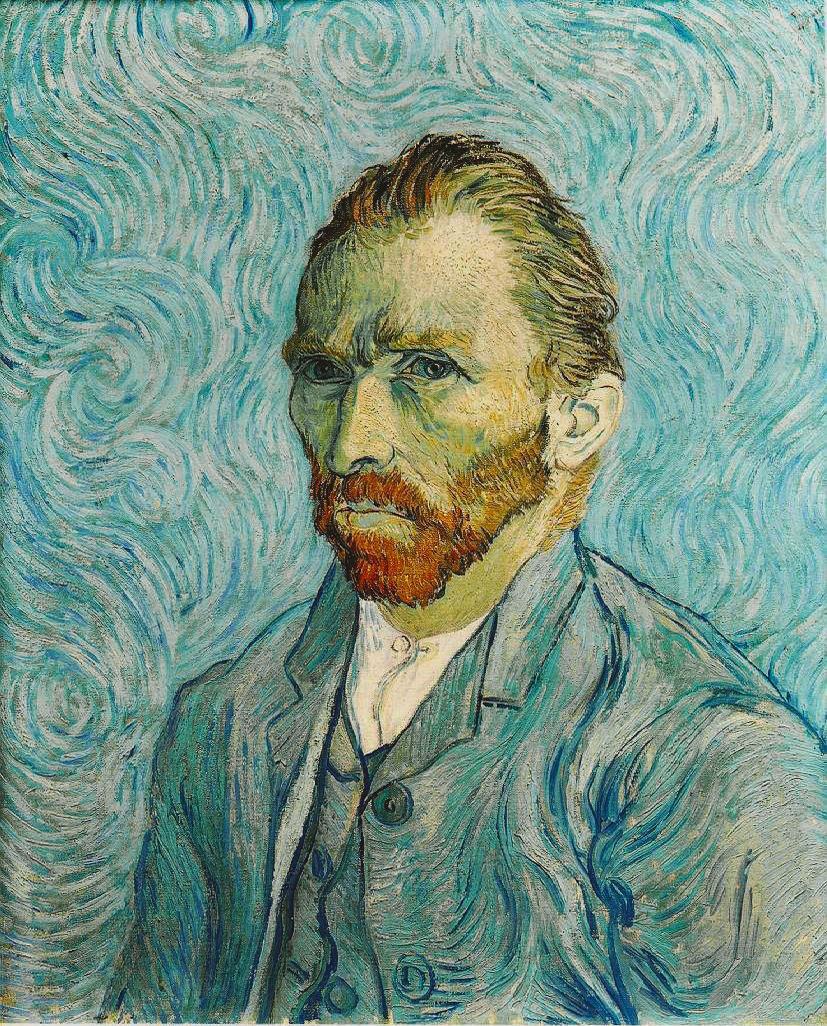
\includegraphics[width=0.4\textwidth]{imagenes/Autorretrato.jpg}
    \caption[Autorretrato, de Van Gogh]{Autorretrato, de Van Gogh (Musée d'Orsay, Paris). Extraído de \cite{Gogh1889}.}
    \label{fig:van_gogh_autorretrato}
\end{figure}

Disfrutó de amistad y admiración con los mejores pintores de su época, reinventando el impresionismo previo de Monet (tanto él como Cézanne son considerado postimpresionistas, si bien por simplificación los incluimos como impresionistas).
Esta evolución se puede ver en los colores vivos, en el abandono del naturalismo en sus composiciones, formas que parecen moverse o caerse (influyendo al posterior surrealismo). \newline

Sus problemas psiquiátricos (con el ingreso de un año en un frenopático después de su incidente con la oreja) no le impidieron componer de forma asombrosa, con cuadros como la serie de \textit{La noche estrellada}. Uno de ellos se muestra en la figura \ref{fig:van_gogh_noche_estrellada}. Se suicidó en 1889 disparándose en el pecho con un revólver \cite{Barreira2019}.

\begin{figure}[h!]
    \centering
    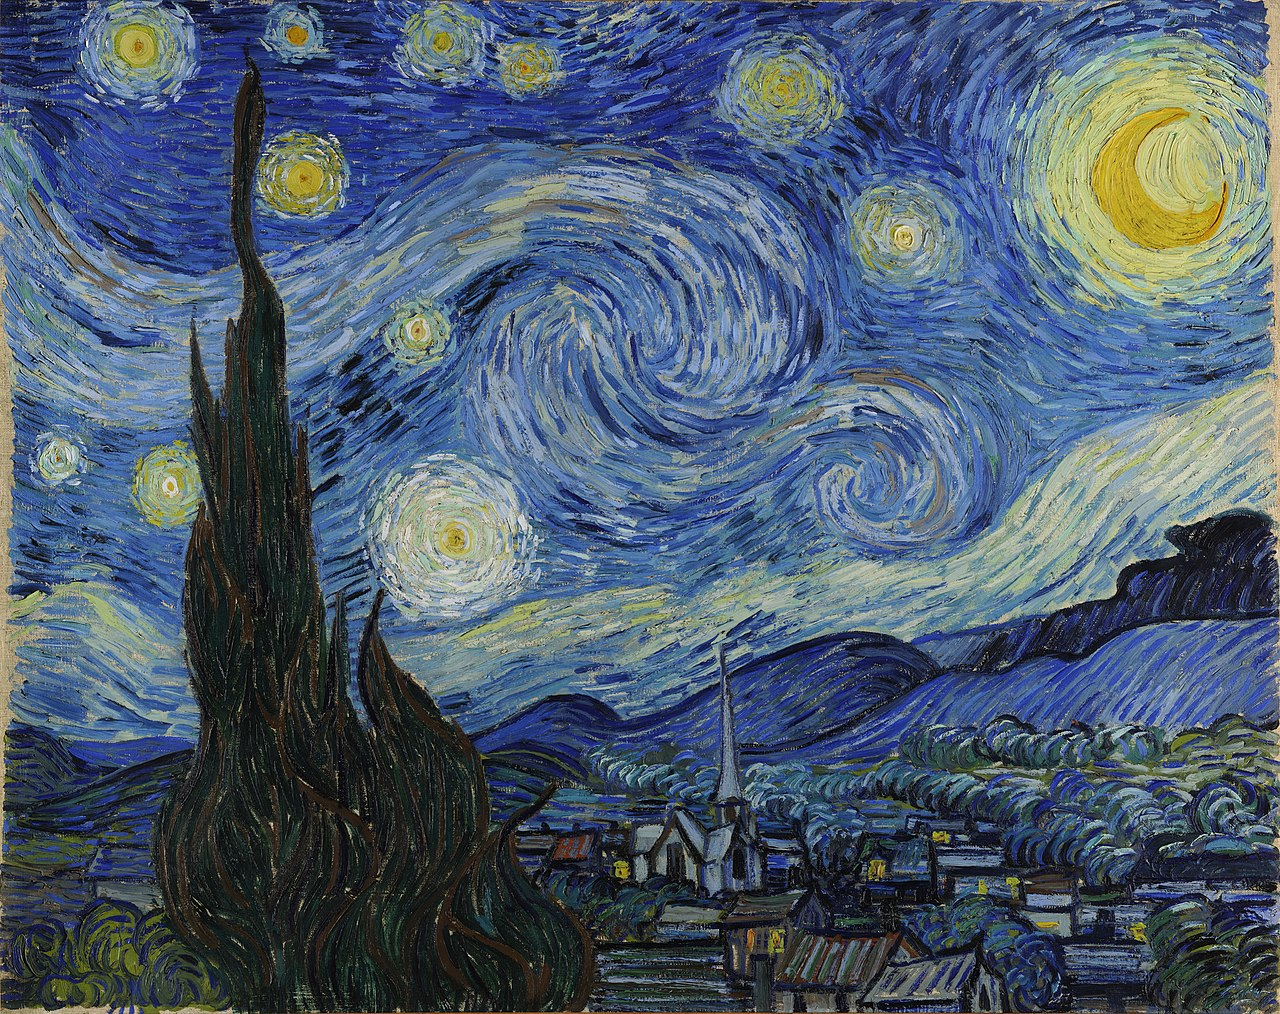
\includegraphics[width=0.6\textwidth]{imagenes/La noche estrellada.JPG}
    \caption[La noche estrellada, de Van Gogh]{La noche estrellada, de Van Gogh (Museum of Modern Art, Nueva York) Extraído de \cite{VanGogh1889}.}
    \label{fig:van_gogh_noche_estrellada}
\end{figure}

\subsection{Cézanne}

Paul Cézanne (1839-1906), pintor francés. Pintor ignorado en vida, apenas expuso y pasó una vida enclavado en la pobreza, con poco reconocimiento en vida \cite{CalvoSantos2016-3}.

\begin{figure}[h]
    \centering
    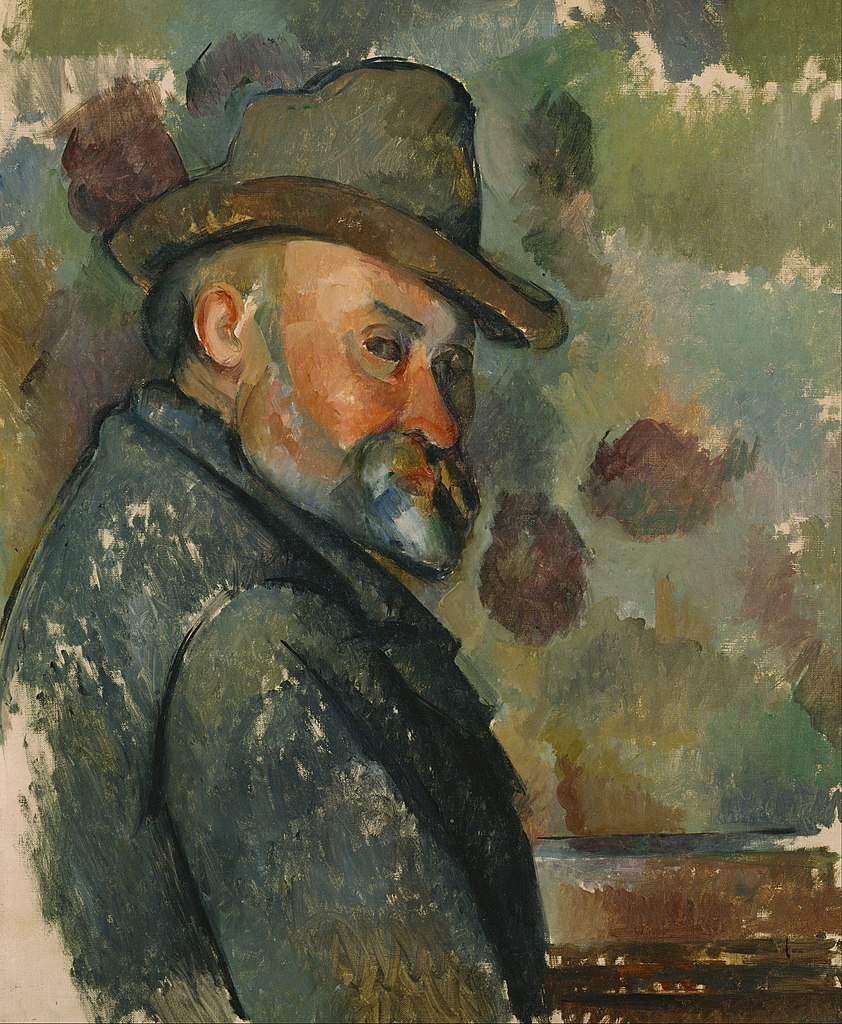
\includegraphics[width=0.4\textwidth]{imagenes/Autorretrato con sombrero arrugado.jpg}
    \caption[Autorretrato con sombrero arrugado, de Paul Cézanne]{Autorretrato con sombrero arrugado, de Paul Cézanne (Bridgestone Museum of Art, Tokio). Extraído de \cite{Cezanne1894}.}
    \label{fig:cezanne_autorretrato}
\end{figure}

Si bien frecuentaba los círculos impresionistas (expuso en 1874 en la exposición inicial del grupo), las críticas que recibieron sus cuadros provocaron que Cézanne no volviese a exponer, comenzando un camino personal. No obstante, hacia el final de su vida volvió a exponer, comenzando a ser su obra valorada e influyendo en los pintores posteriores \cite{ElizaldeOcampo2020}.\newline
Con el paso del tiempo, sus cuadros empezaron a ser muy valorados. Su cuadro más famoso, \textit{Los jugadores de cartas} (figura \ref{fig:cezanne_cartas}) del año 1893 , fue adquirido por la familia real de Catar por 250 millones de dólares (191,6 millones de euros) en 2011 \cite{EFE2016}. \newline

\begin{figure}[h]
    \centering
    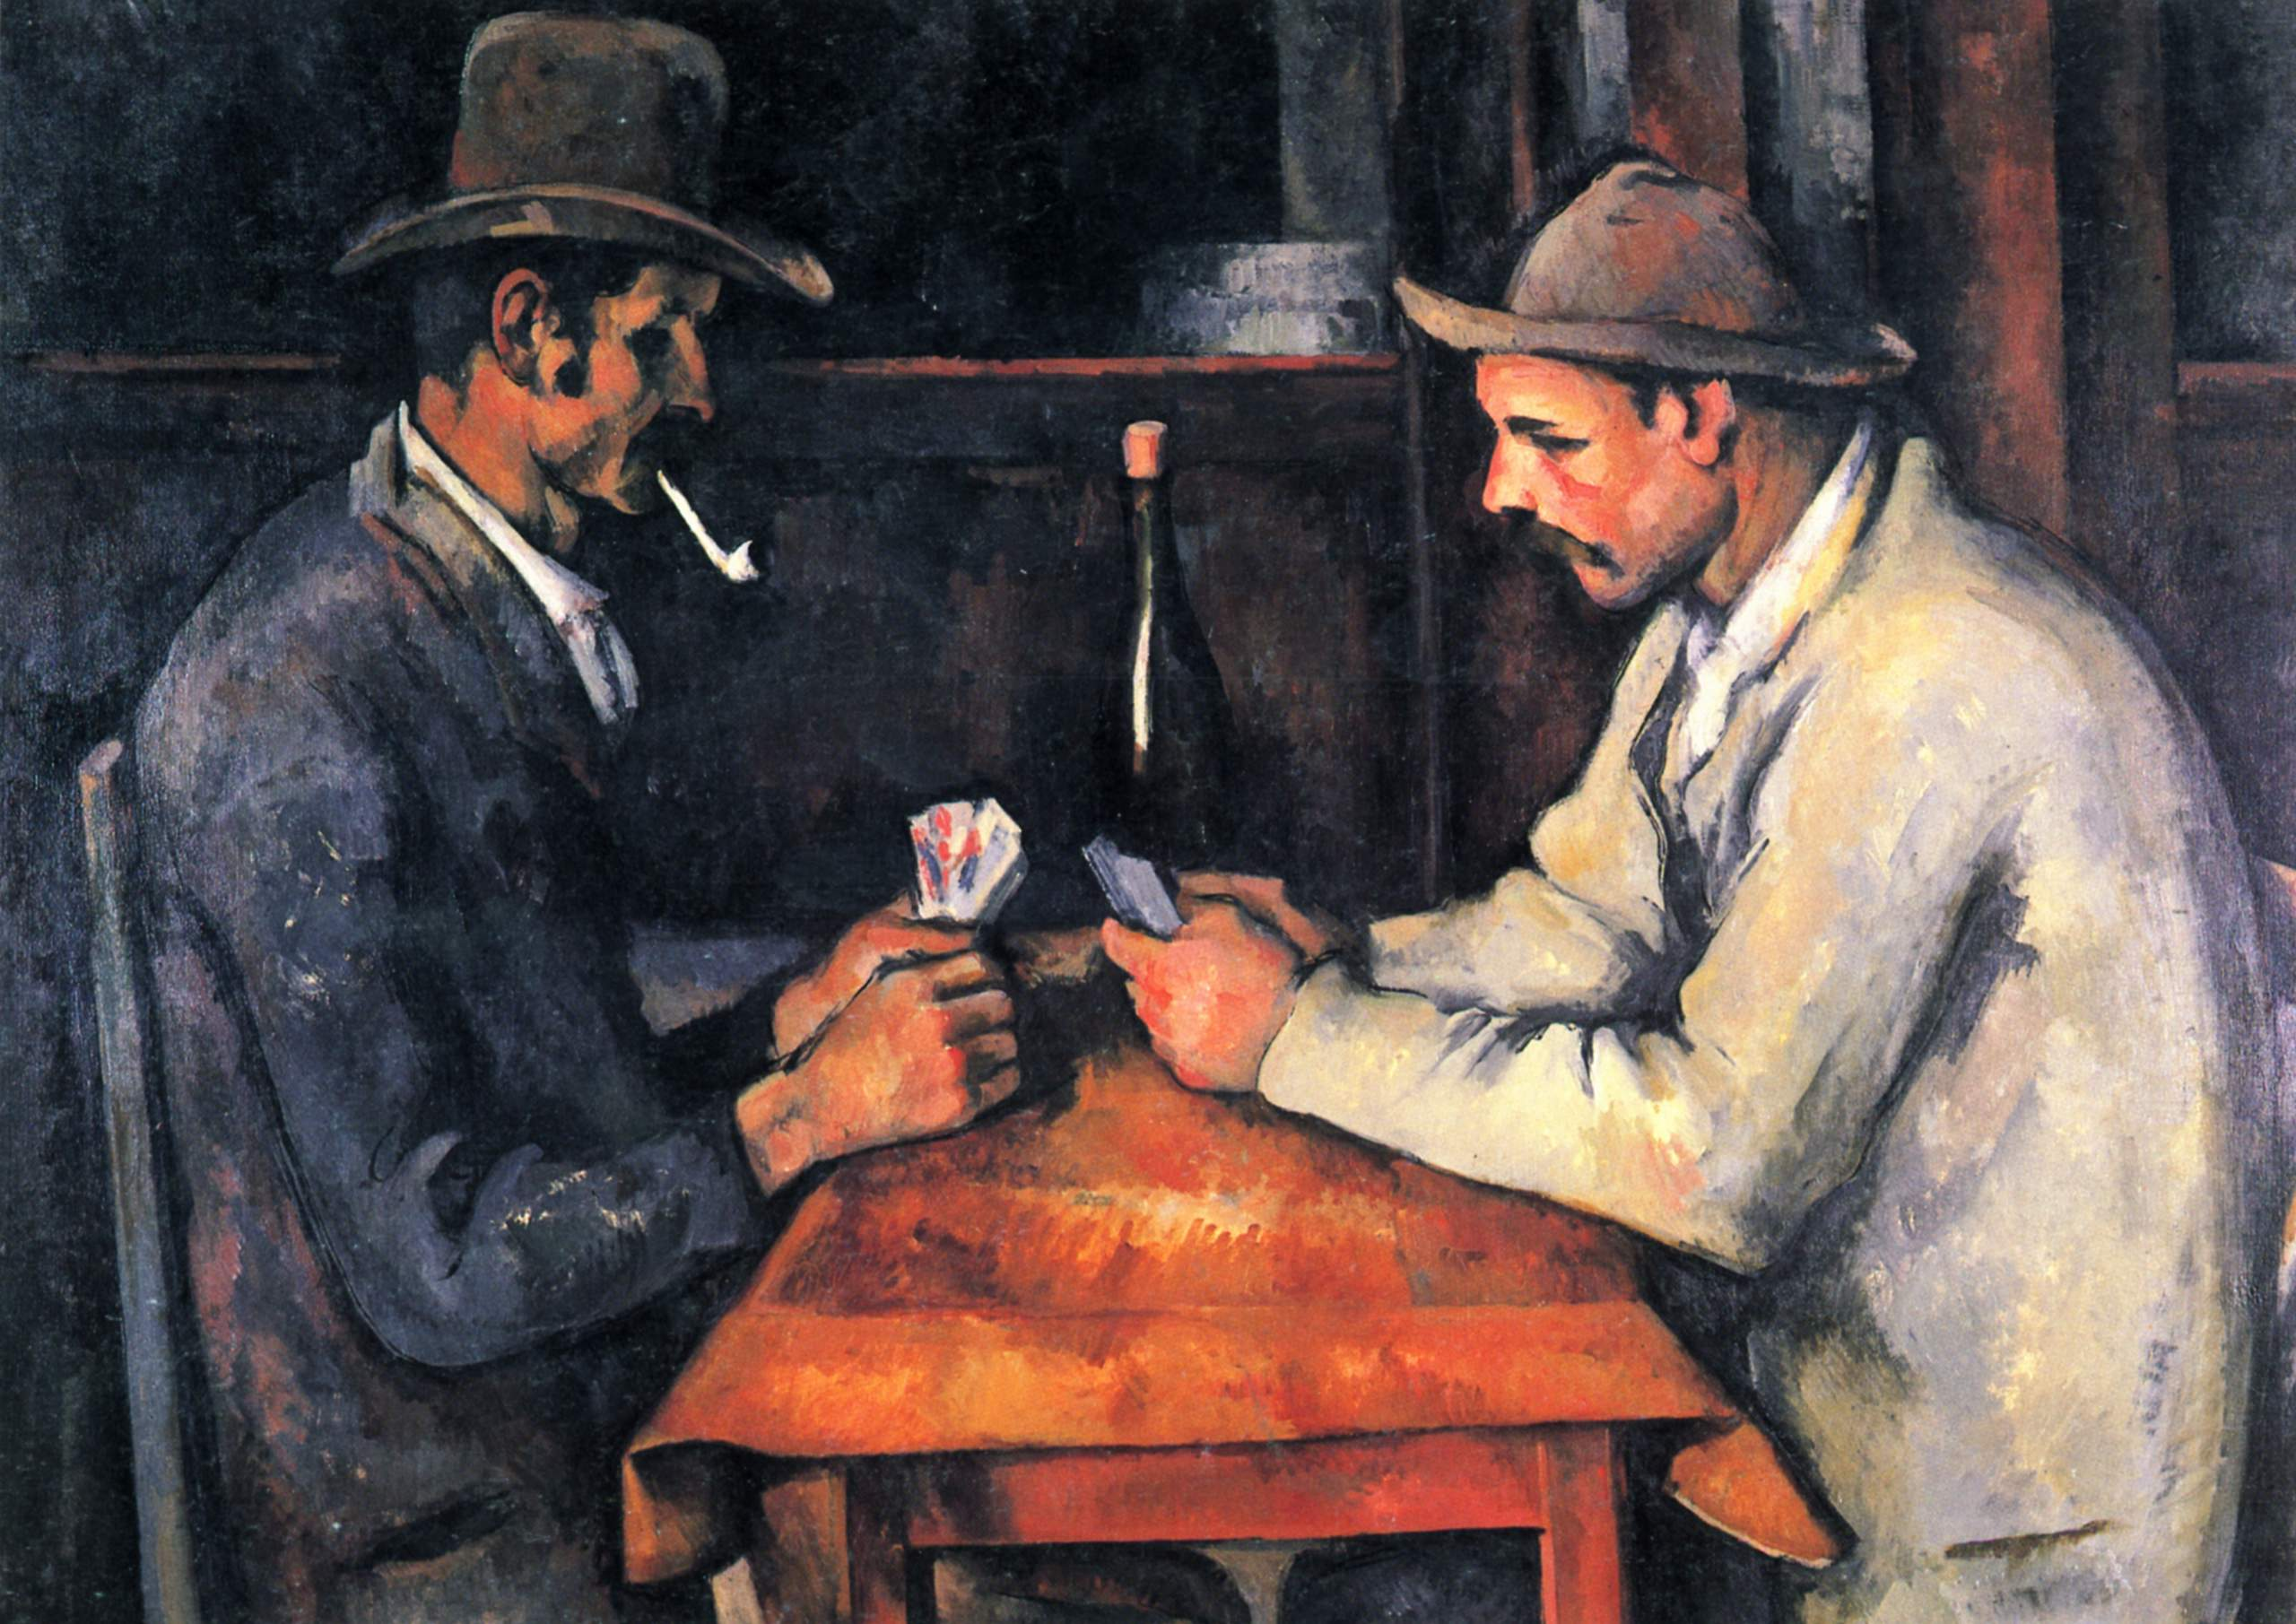
\includegraphics[width=0.6\textwidth]{imagenes/Los jugadores de cartas.jpg}
    \caption[Los jugadores de cartas, de Paul Cézanne]{Los jugadores de cartas, de Paul Cézanne (Colección privada de la familia real catarí). Extraído de \cite{Cezanne1893}.}
    \label{fig:cezanne_cartas}
\end{figure}

A diferencia de Monet y Van Gogh, Cézanne intentó aunar en sus obras el orden, la expresión personal y el naturalismo, estructurando la obra en formas simples y planos de color. Esto lo conseguía representando de la forma más exacta posible desde el punto de vista pictórico, con pinceladas muy particulares con las que representa simultáneamente lo que el ojo que observa y una abstracción de eso, es decir, perspectivas diferentes al mismo momento. Esta simultaneidad sería adoptada posteriormente por los pintores cubistas \cite{CalvoSantos2016-3}.

 \begin{center}
    \begin{minipage}{0.9\linewidth}
        \vspace{5pt}%margen superior de minipage
        {\small
            ¡Cézanne es mi único y singular maestro!
        }
        \begin{flushright} Pablo Picasso en 1964 \cite{WikiquoteCezanne}
        \end{flushright}
        \vspace{1pt}%margen inferior de la minipage
    \end{minipage}
\end{center}

\section{Inteligencia Artificial y Redes Neuronales}
\subsection{¿Qué es la Inteligencia Artificial?}
La Inteligencia Artificial es un concepto con numerosas definiciones e interpretaciones, por lo que no se pretende en este documento hacer un estudio extenso y profundo de la misma ya que se escapa a los límites y objetivos de este Trabajo Final de Grado. Para ampliar sobre este tema se recomienda acudir a la bibliografía citada en esta sección. \newline
A la hora de definir la inteligencia artificial cabe esperar que primero haya que clarificar qué entendemos por inteligencia. Una de las muchas definiciones que tiene inteligencia es la siguiente:

 \begin{center}
    \begin{minipage}{0.9\linewidth}
        \vspace{5pt}%margen superior de minipage
        {\small
            Habilidad para responder flexiblemente a diferentes situaciones, saber aprovechar circunstancias fortuitas, dar sentido a mensajes ambiguos o contradictorios, encontrar similitudes entre situaciones diferentes y generación de nuevos conceptos e ideas innovadoras.
        }
        \begin{flushright} Douglas Hofstadter \cite{Garcia2012}
        \end{flushright}
        \vspace{3pt}%margen inferior de la minipage
    \end{minipage}
\end{center}

Basándonos en esa definición, podemos describir la inteligencia artificial de la siguiente manera:

 \begin{center}
    \begin{minipage}{0.9\linewidth}
        \vspace{5pt}%margen superior de minipage
        {\small
            El arte de crear máquinas que realicen funciones que requerirían inteligencia si fueran realizadas por humanos.
        }
        \begin{flushright} Raymond Kurzweil \cite{Garcia2012}
        \end{flushright}
        \vspace{3pt}%margen inferior de la minipage
    \end{minipage}
\end{center}

Una vez clarificado qué entendemos por Inteligencia Artificial, podemos ver que el concepto es bastante amplio, por lo que se puede subdividir el concepto en diferentes niveles para ayudar a situarnos \cite{Pastor2018}:

\begin{itemize}
    \item Inteligencia artificial débil: este tipo de inteligencia es capaz de resolver problemas muy bien definidos y acotados. En esta división es donde se enmarcan los progresos hasta la fecha en el campo, mediante técnicas como el \textit{machine learning} (aprendizaje máquina) y \textit{deep learning} (aprendizaje profundo) para resolver problemas específicos. Se ha conseguido que estos sistemas acaben realizando esas tareas mucho más rápido (y en ocasiones mejor) que un ser humano, pero no son capaces de adaptarse a su entorno. Este Trabajo de Fin de Grado se ubica en esta sección.
    \item Inteligencia artificial general: esta inteligencia artificial, aún inexistente, permitiría resolver cualquier tarea intelectual resoluble por un ser humano, es decir, sería multitarea como los humanos. No sería únicamente una concatenación de inteligencias artificiales débiles, ya que además sería capaz de realizar juicios, razonar ante la incertidumbre, planificar y aprender.
    \item Inteligencia artificial fuerte: añadiría a la general la consciencia de sí misma, muy en la línea de \textit{Skynet} y las demás inteligencias artificiales planteadas por el cine. Teóricamente sería capaz de resolver cualquier problema y sentiría emociones.
\end{itemize}

\subsection{Fundamentos de Machine Learning}

El \textit{Machine Learning} (o Aprendizaje Automático en castellano) es un paradigma en el que el programador no indica las reglas que debe ejecutar el programa, sino que suministra los datos a tratar y (en ocasiones) las respuestas deseadas; y el sistema debe aprender las reglas que resuelven el problema. \newline
Este proceso se repite durante un número concreto de veces (llamado \textit{epoch}), para posteriormente evaluar el modelo en otro conjunto de datos (independiente del primero), llamado conjunto de test, de acuerdo a unas métricas. \newline
En ocasiones se posee un tercer conjunto (independiente de los dos anteriores), llamado conjunto de validación, sobre el que se realiza una evaluación con el modelo \textit{más refinado posible} para comprobar si es válido en la vida real y si es así ponerlo a funcionar.

Por otra parte, el proceso mediante el cual el sistema aprende se puede dividir en cuatro tipos:

\begin{itemize}
    \item Aprendizaje supervisado: el programador proporciona al sistemas un conjunto de datos, para las que se conoce tanto la entrada como la salida. Un ejemplo de este tipo son los filtros de spam.
    
    \item Aprendizaje no supervisado: en este caso el sistema conoce las entradas pero no las salidas del mismo. Se suele utilizar para comprender, entender o eliminar datos (\textit{clustering}) y para visualización y reducción de dimensionalidad (Análisis por Componentes Principales).
    
    \begin{figure}[h]
        \centering
        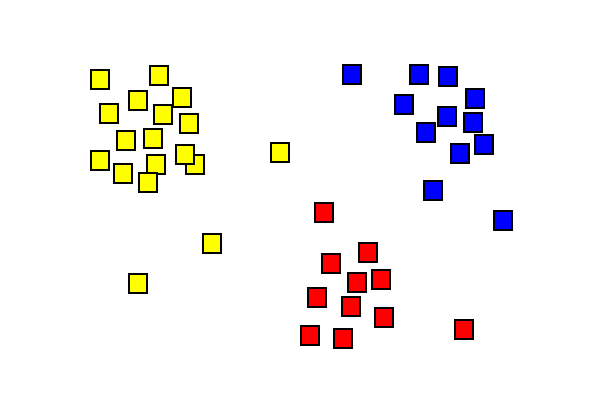
\includegraphics[width=0.4\textwidth]{imagenes/Clustering.png}
        \caption[Ejemplo de clustering.]{Ejemplo de clustering. Imagen de dominio público.}
        \label{fig:ejemplo_clustering}
    \end{figure}
    
    \item Aprendizaje semisupervisado: en lugar de disponer para cada dato su salida esperada (o no disponer de ella), se tienen los dos casos. Si bien suena extraño, hay ejemplos en nuestra vida cotidiana: servicios como Google Fotos pueden detectar las personas presentes en una galería de fotos, pero el usuario debe decirle al sistema quién es \cite{Geron2019}. La mayoría de estos algoritmos suelen ser mezcla de modelos supervisados y no supervisados, como en el caso de las \textit{Deep Belief Networks}.
    
    \item Aprendizaje por refuerzo: en este caso, el sistema (o agente en la literatura de este campo) observa el entorno y realiza una serie de decisiones, por las que recibe una recompensa (puede ser negativa). En este caso, el agente tiene que aprender cuál es la mejor estrategia para maximizar la recompensa obtenida. Este tipo de aprendizaje se aplicó en la máquina AlphaGo (de la que hablamos en la introducción), o en algo mucho más común como el adiestramiento de una mascota. 
    
\end{itemize}

\subsection{¿Por qué usar Machine Learning?}

Para dar convencer al lector, usaré el ejemplo mostrado en \cite{Geron2019}. Supongamos que queremos realizar un sistema de detector de spam mediante programación tradicional, el cual no dispone de una solución cerrada mediante un algoritmo. Seguiríamos el siguiente proceso para realizar el programa:

\begin{enumerate}
    \item Analizaríamos los rasgos que presentan los mensajes de spam. Podríamos empezar con palabras tales como \"tarjeta de crédito\", \"gratis\" y \"alucinante\", para posteriormente complicar el sistema incluyendo reglas sobre el nombre del emisor, el cuerpo del mensaje...
    \item Implementaríamos dichos rasgos en un programa que tomase un correo y ejerciese de filtro, indicando si el filtro es (o no) spam.
    \item Testearíamos el programa y repetiríamos los pasos 1 y 2 hasta que el programa sea lo \textit{suficientemente bueno}.
\end{enumerate}

Debido a la complejidad del problema, el conjunto de reglas del problema sería cada vez mayor y más complicado, siendo difícil de mantener. En contrapartida, un sistema basado en aprendizaje automático captaría los patrones de palabras y párrafos propios de los mensajes de spam, por lo que el programa sería mucho más fácil de desarrollar y mantener.\newline

Una vez lanzásemos nuestro programa, las personas que envían spam se darían cuenta de qué palabras bloquean sus mensajes, por lo que modificarían los mismos para saltarse nuestro filtro, por lo que tendríamos que reescribir las reglas indefinidamente. Sin embargo, el sistema basado en \textit{Machine Learning} aprendería las nuevas técnicas de los \textit{spammers} sin nuestra intervención, ahorrando desarrollo y problemas al programador. \newline

\begin{figure}[h]
    \centering
    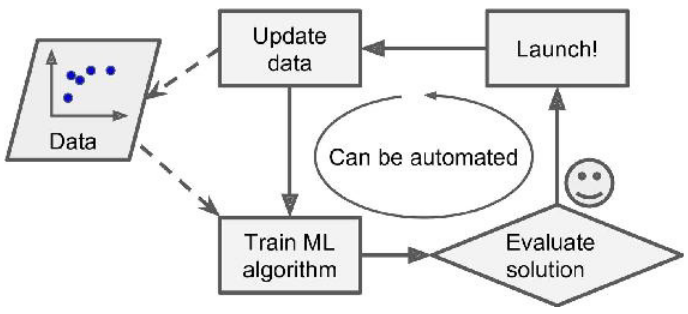
\includegraphics[width=0.6\textwidth]{imagenes/Ciclo vida ML.png}
    \caption[Ciclo de vida de una aplicación de Machine Learning.]{Ciclo de vida de una aplicación de Machine Learning. Tomado de \cite{Geron2019}.}
    \label{fig:ciclo_vida_ml}
\end{figure}

Este enfoque se puede extender a todos los problemas que no disponen de una solución algorítmica sencilla: donde un programa tradicional tendría que desarrollar un algoritmo con reglas muy concretas y focalizadas para cada casuística, un sistema de aprendizaje automático puede reconocer esos patrones para todo el conjunto de datos del que dispongamos. Este descubrimiento de patrones nos permite detectar correlaciones poco imaginables a priori, además de nuevas tendencias, lo que nos permite entender mejor nuestro problema. Este último concepto se conoce como Minería de Datos. \newline

No obstante, dentro del Machine Learning también existen problemas. Entre ellos destacamos :
\begin{itemize}
    \item Cantidad insuficiente de datos: a diferencia de los humanos, las máquinas no aprenden únicamente con un sólo ejemplo, necesitan ver miles o millones de ejemplos durante cientos de veces para aprender. Disponer de pocos datos produce ruido muestral, entre otros fenómenos.
    \item Sesgos en la elaboración del conjunto de datos y/o incompletitud del mismo. Como en nuestra vida, si disponemos de datos sesgados y/o incompletos no podemos realizar razonamientos correctos.
    \item Overfitting o sobreajuste: existe el riesgo de que el modelo pierda la capacidad de generalizar y que simplemente se aprenda el conjunto de entrenamiento. Por este fenómeno se elige el modelo mediante sus resultados en el conjunto de test. Puede mitigarse reduciendo el número de parámetros del modelo y/o aumentando la cantidad de datos y/o la calidad de los mismos.
    
    \begin{figure}[h]
        \centering
        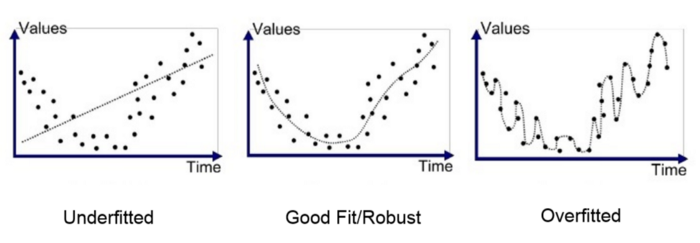
\includegraphics[width=0.85\textwidth]{imagenes/Under-overfitting.png}
        \caption[Ejemplo de underfitting, ajuste óptimo y overfitting.]{Ejemplo de underfitting, ajuste óptimo y overfitting. Extraída de \cite{Balaji2019}}
        \label{fig:ejemplo_underfitting_overfitting}
    \end{figure}
    
    \item Underfitting o infrajuste: el sistema es incapaz de aprender y generalizar. Ocurre al seleccionar un modelo demasiado simple, aunque también puede ocurrir si las características que utilza el modelo para aprender son poco potentes.
\end{itemize}

\subsection{¿Qué son las Redes Neuronales?}

Una red neuronal es un sistema computacional inspirado en las neuronas biológicas que cada uno disponemos en nuestro cerebro, creado por los investigadores Warren McCulloch y Walter Pitts en 1943 \cite{PonceCruz2010}. \newline

Una neurona artificial se compone de neuronas y conexiones, siendo la neurona "aislada" un equivalente artificial a las dentritas y axones; mientras que el enlace simula la sinapsis biológica al interconectar varias neuronas en un enlace de 1 a varios (la salida de una neurona se interconecta a cierto número de neuronas) \cite{SerradillaGarcia2016}. Matemáticamente la neurona realiza la siguiente operación:

\begin{equation}
    y = \sigma(\sum_{i=1}^{n}(x_{i}\cdot \omega_{i}) + b)
    \label{eq:fundamental_neurona}
\end{equation}

donde $y$ es la salida de la neurona, $\sigma$ es la función de activación de la neurona, $x_{i}$ es la entrada $i$-ésima de la neurona, $\omega_{i}$ es el peso (ponderación) del enlace de la neurona $i$-ésima y $b$ representa al término \textit{bias}, un parámetro por el cual el modelo puede desplazar o ajustar una función de activación sin transformar su forma por completo.

\begin{figure}[h]
    \centering
    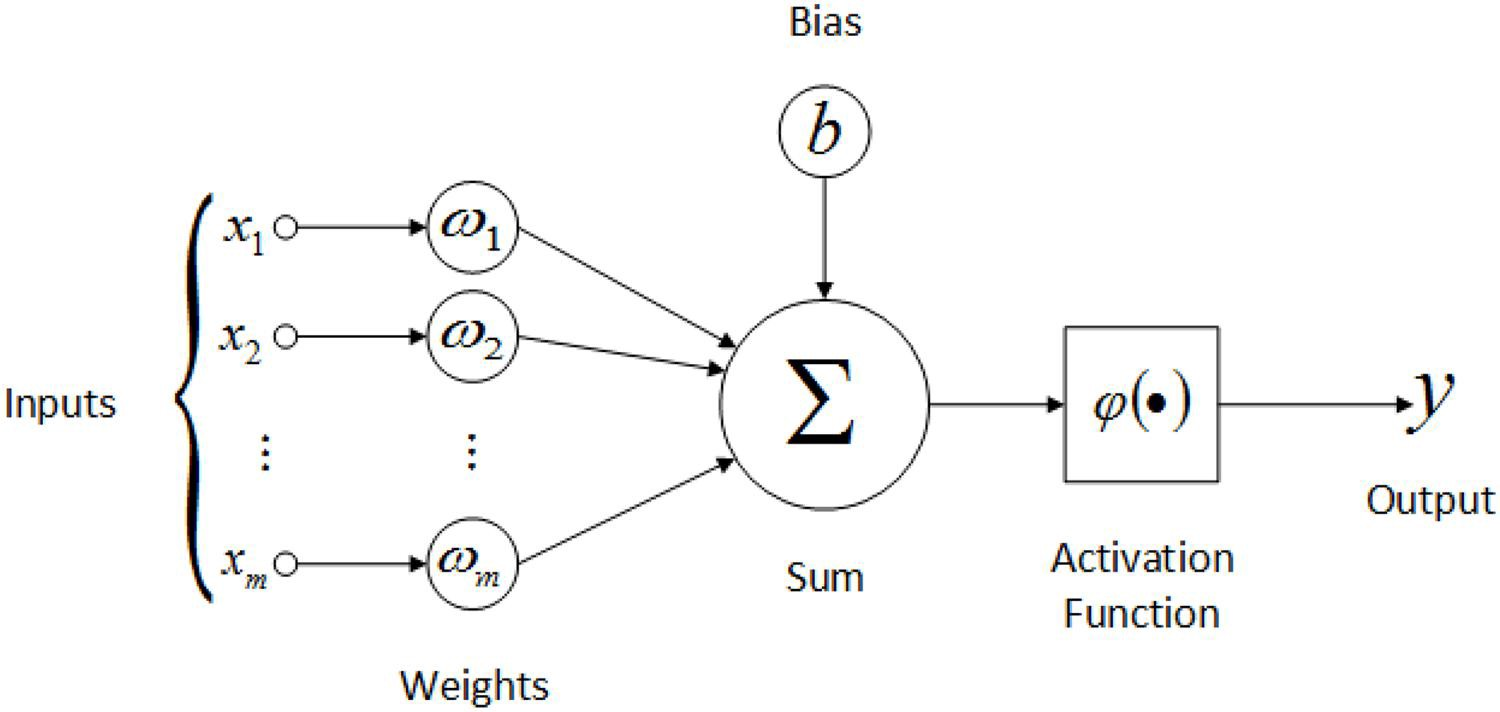
\includegraphics[width=0.85\textwidth]{imagenes/Neurona.jpeg}
    \caption[Representación gráfica de la función de una neurona artificial.]{Representación gráfica de la función de una neurona artificial realizando la ecuación \ref{eq:fundamental_neurona}. Extraída de \cite{Mendoza2019}.}
    \label{fig:neurona_artificial_proceso}
\end{figure}

Ampliemos ahora el significado de algunos elementos de la ecuación \ref{eq:fundamental_neurona}:

\subsubsection{Pesos de los neuronas y algoritmo básico de aprendizaje}
Los pesos de las neuronas ($\omega_{i}$) son números reales, utilizados por el modelo para su ajuste, inicializándose aleatoriamente. El método por el cual la neurona aprende los valores correctos de los pesos es minimizando la función pérdida, que mide la diferencia entre la salida esperada y la salida actual. Dicha diferencia puede calcularse mediante muchas funciones, como la función \textit{Root Mean Square Error} (RMSE).

\begin{equation}
    RMSE = \sqrt{\frac{1}{N}  \cdot \sum_{n=1}^{N} (d_n - s_n)^2}
\end{equation}

El ajuste de los pesos como tal es realizado por un algoritmo llamado optimizador, uno de los parámetros del modelo que determina el programador. Los más conocidos son el algoritmo clásico de \textit{backpropagation} (retropropagación en inglés), que se basa en el método \textit{descenso del gradiente} y ADAM , basado en \textit{backpropagation} y en otros muchos. En este Trabajo Fin de Grado se utiliza ADAM debido a sus ventajas sobre otros optimizadores \cite{kingma2017adam}. \newline
Por otra parte, los pesos son actualizados en cada iteración proporcionalmente a un parámetro llamado $\mu$ (ajustado por el programador) conocido como ratio de aprendizaje. Una vez modificados los pesos se realiza una nueva iteración con otros datos del conjunto de entrenamiento. Una vez se pasa por todos los datos, se vuelve a iterar sobre el mismo, así hasta alcanzar un número fijado de veces llamado \textit{epoch}.

\subsubsection{Funciones de activación}
La función de activación (que puede ser cualquier tipo de función) es la encargada de introducir relaciones no lineales entre las variables de entrada y la de salida. Es un parámetro que también es fijado por el programador, ya que dependiendo de la tarea a realizar algunas tienen mejor desempeño que otras. Presentamos algunas de las más conocidas \cite{Kzrak2019}:


\begin{table}[h]
\begin{tabular}{|l|l|l|}
 \hline
Función                      & Expresión & Rango \\
 \hline
Lineal                      & $f(x)=x$  &  $(-\infty,\infty)$     \\
 \hline
Escalón                       & $f(x)=$ \left\{\begin{array}{lcc}
                                            0 &   si  & x \leq 0 
                                            \\ 1 &  si  & x \geq 0
                                            \end{array}
                                             \right.          &      $(0,1)$     \\
 \hline
Sigmoidal                    &  $f(x)=\ddfrac{1}{1 + e^{-x}}$      &    $(0,1)$   \\
 \hline
ReLU (Rectified Linear Unit) &   $f(x)=$ \left\{\begin{array}{lcc}
                                            0 &   si  & x \leq 0
                                            \\ x &  si  & x \geq 0
                                            \end{array}
                                             \right.           &    $[0, \infty)$  \\
 \hline
Leaky-ReLU                   &  $f(x)=$ \left\{\begin{array}{lcc}
                                            0.01 &   si  & x \leq 0
                                            \\ 1 &  si  & x \geq 0
                                            \end{array}
                                             \right.            &  $(-\infty,\infty)$     \\
\hline
\end{tabular}
\caption{Comparación entre algunas de las funciones de activación más populares}
\label{ta:funciones_activacion}
\end{table}

\subsubsection{Concepto de capa y de Red Neuronal Profunda}

Hasta ahora sólo habíamos hablado de una neurona, sin tener en cuenta la arquitectura de la red a la cual pertenece. Existen dos categorías principales de estructuras de redes neuronales: acíclicas o redes con alimentación-hacia-delante y cíclicas o redes recurrentes \cite{Rusell2004}. Las primeras son las que explicamos en \ref{eq:fundamental_neurona}, y las redes recurrentes se caracterizan porque las entradas dependen de sus salidas en un estado anterior, lo que las hace disponer de memoria a corto plazo pero son mucho más complicadas de entender, programar y entrenar, por lo que están fuera del alcance de este \tfg. 

Las redes neuronales con alimentación hacia delante normalmente se organizan en capas, de forma que cada unidad recibe entradas únicamente de las unidades de la capa que la precede inmediatamente \cite{Rusell2004}. A las redes neuronales que sólo tienen una capa de entrada y otra de salida se les conoce como perceptrones. \newline

El problema de los perceptrones es que sólo pueden aprender funciones lineas, y para que una red neuronal pueda aprender funciones no lineales (algunas tan simples como la XOR) es necesario incluir una o más capas intermedias, llamadas capas ocultas \cite{Hilton1986}. A las redes con una o más capas ocultas se les conoce como Redes Neuronales Profundas. \newline

En la figura \ref{fig:perceptron_profunda} se puede ver visualmente la diferencia, siendo la capa morada de la capa oculta.

\begin{figure}[h]
    \centering
    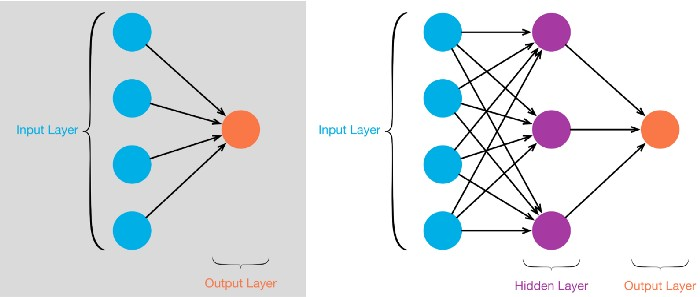
\includegraphics[width=1\textwidth]{imagenes/Red sin oculta vs red con oculta.jpeg}
    \caption[Perceptrón y Red Neuronal Profunda]{Perceptrón y Red Neuronal Profunda. Tomado de \cite{Kang2017}.}
    \label{fig:perceptron_profunda}
\end{figure}

\subsection{¿Por qué usar Redes Neuronales?}

Las Redes Neuronales son adecuadas para aquellos problemas que no tienen una solución computacional precisa o que requieren algoritmos muy extensos \cite{PonceCruz2010}. El problema que queremos resolver en este Trabajo Fin de Grado no tiene solución mediante un algoritmo sencillo y preciso, por lo que de primeras parecen adecuadas. Asimismo, las Redes Neuronales presentas las siguientes ventajas \cite{SerradillaGarcia2016}:

\begin{itemize}
    \item Están basadas en la inducción y la generalización. Aprenden de la experiencia.
    \item Se adaptan muy bien a la computación en paralelo, permitiendo una gran escalabilidad en problemas complejos.
    \item Autoorganización: crean su propia representación de la información que reciben durante el entrenamiento.
    \item Tolerancia a fallos: pueden trabajar con información parcial debido a que codifican la información de modo distribuido y redundante.
    \item Flexibilidad: pueden adaptarse a un nuevo entorno sin necesidad de ser reprogramadas, gracias a su capacidad de aprendizaje
\end{itemize}

No obstante, las redes neuronales también presentan desventajas:

\begin{itemize}
    \item Elecciones de arquitectura y parámetros por ensayo y error si no hay estudios previos sobre problemas similares.
    \item Aprendizaje lento y dificultoso.
    \item Ausencia de explicación de las decisiones, lo que impide que comprendamos correctamente qué hace el sistema.
\end{itemize}

Podemos concluir que al elegir una red neuronal, no obtendremos muchos datos sobre cómo aprende el sistema y cómo representa la información internamente, pero tendremos una modelo que si lo conseguimos entrenar correctamente será eficiente y podrá aprender los estilos de Cézanne, Monet y Van Gogh programándolas una sola vez.

\subsection{Redes Neuronales Convolucionales}

Las Redes Neuronales Convoluciones son un tipo de red neuronal inspirada en la corteza visual que hay en los cerebros biológicos. Simplificando mucho, en la capa primaria o V1 de la corteza visual, tenemos células que reconocen patrones elementales (lineas horizontales y verticales) y que sólo se activan si lo reconocen \cite{Hubel1959}. Matemáticamente ese tipo de reconocimiento forma parte de una operación más genérica, llamada convolución (de ahí su nombre). \newline

Las siguientes capas (V2, V3...) están conectadas a la salida de la capa inmediatamente anterior, reconociendo patrones cada vez más complejos \cite{Geron2019}. Esto inspiró a Kunihiko Fukushima, quien presentó en 1980 el Neocognitron \cite{Fukushima1980}, que gradualmente evolucionó hasta las redes neuronales convolucionales de hoy día. \newline

\begin{figure}[h]
    \centering
    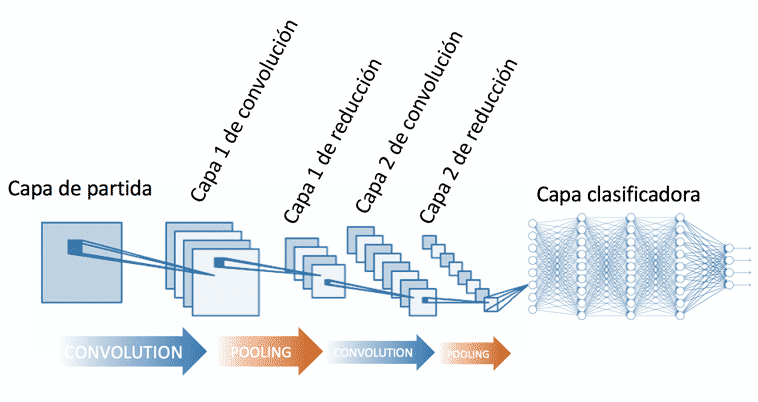
\includegraphics[width=0.6\textwidth]{imagenes/red-neuronal-convolucional-arquitectura.png}
    \caption[Arquitectura de una RNC]{Arquitectura de una RNC. Tomada de \cite{Calvo2017}.}
    \label{fig:arquitectura_convolucional}
\end{figure}

La idea principal de estas redes es que cada neurona de la capa de entrada aprende a reconocer un tipo de patrón sencillo, para que la siguiente capa, a partir de los resultados de la capa precedente, aprenda un patrón un poco más complejo que el anterior. Este estructura jerárquica es muy común en las imágenes reales, por lo que las RNC funcionan muy bien en el reconocimiento de imágenes \cite{Geron2019}. Finalmente, podemos definir que una red convolucional es una red profunda que consta de capas convolucionales y de reducción alternadas, con una capa de salida que realiza una convolución especial que \textit{aplana} la matriz anterior (pasamos de una matriz multidimensional a una unidimensional). 

\subsubsection{¿Qué es la convolución en reconocimiento de imágenes?}

La operación de convolución extrae partes del mapa de entrada (el primer mapa es la propia imagen) y realiza una transformación a todos las secciones, produciendo un mapa de salida. Esta transformación consiste en multiplicar el mapa de entrada (que no deja de ser una matriz) por otras pequeñas matrices, denominadas kernel (filtro). \newline

Este kernel se aplica a todas las neuronas de entrada (\textit{deslizando una ventana}, marcada en rojo en la figura \ref{fig:convolución}), generando una matriz de salida llamado mapa de características. Posteriormente a este mapa de salida se le aplica una función de activación, como la ReLU o la Leaky ReLU que expusimos en la tabla \ref{ta:funciones_activacion}. 

\begin{figure}[h]
    \centering
    \includegraphics[width=0.7\textwidth]{imagenes/convolución.png}
    \caption[Operación de convolución]{Operación de convolución]. Tomado de \cite{Calvo2017}.}
    \label{fig:convolución}
\end{figure}

Cabe mencionar que los kernel no son fijos, sino que son aprendidos por la red neuronal, es decir, los valores de los kernel son los valores $\omega_{i}$ de la ecuación \ref{eq:fundamental_neurona}

\subsubsection{¿Qué es la reducción en reconocimiento de imágenes?}

La reducción es una operación muy sencilla: para una matriz de entrada queremos reducir su dimensionalidad. Para ello dividimos la matriz en pequeñas submatrices a las que les realizamos una operación, como pueda ser la media o el valor máximo.\newline 

\begin{figure}[h]
    \centering
    \includegraphics[width=0.6\textwidth]{imagenes/reducción.png}
    \caption[Operación de reducción]{Operación de reducción. Tomado de \cite{Calvo2017}.}
    \label{fig:reducción}
\end{figure}

Si usamos la operación valor máximo, prevalecen las características más importantes del filtro, reduciendo el tamaño del mapa a la mitad o más, reduciendo el número de pesos a aprender. Dicha operación se conoce como \textit{max pooling}, representada en la figura \ref{fig:reducción}

\subsection{Redes Generativas Antagónicas}

Las Redes Generativas Antagónicas, también conocidas como \textit{Generative Adversative Network}) o por sus siglas en inglés GAN (así serán nombradas de ahora en adelante) es un tipo de red neuronal bastante reciente (2014) \cite{Goodfellow2014}, pero al mismo tiempo muy conocida debido a su inmenso potencial. Mucho se ha hablado de ellas por su concepto transgresor y revolucionario, ya que permite dotar a las redes neuronales de cierta \textit{creatividad}. La figura \ref{fig:imagenes_gan} muestra 15 rostros generados por una red GAN. \newline

\begin{figure}[h]
    \centering
    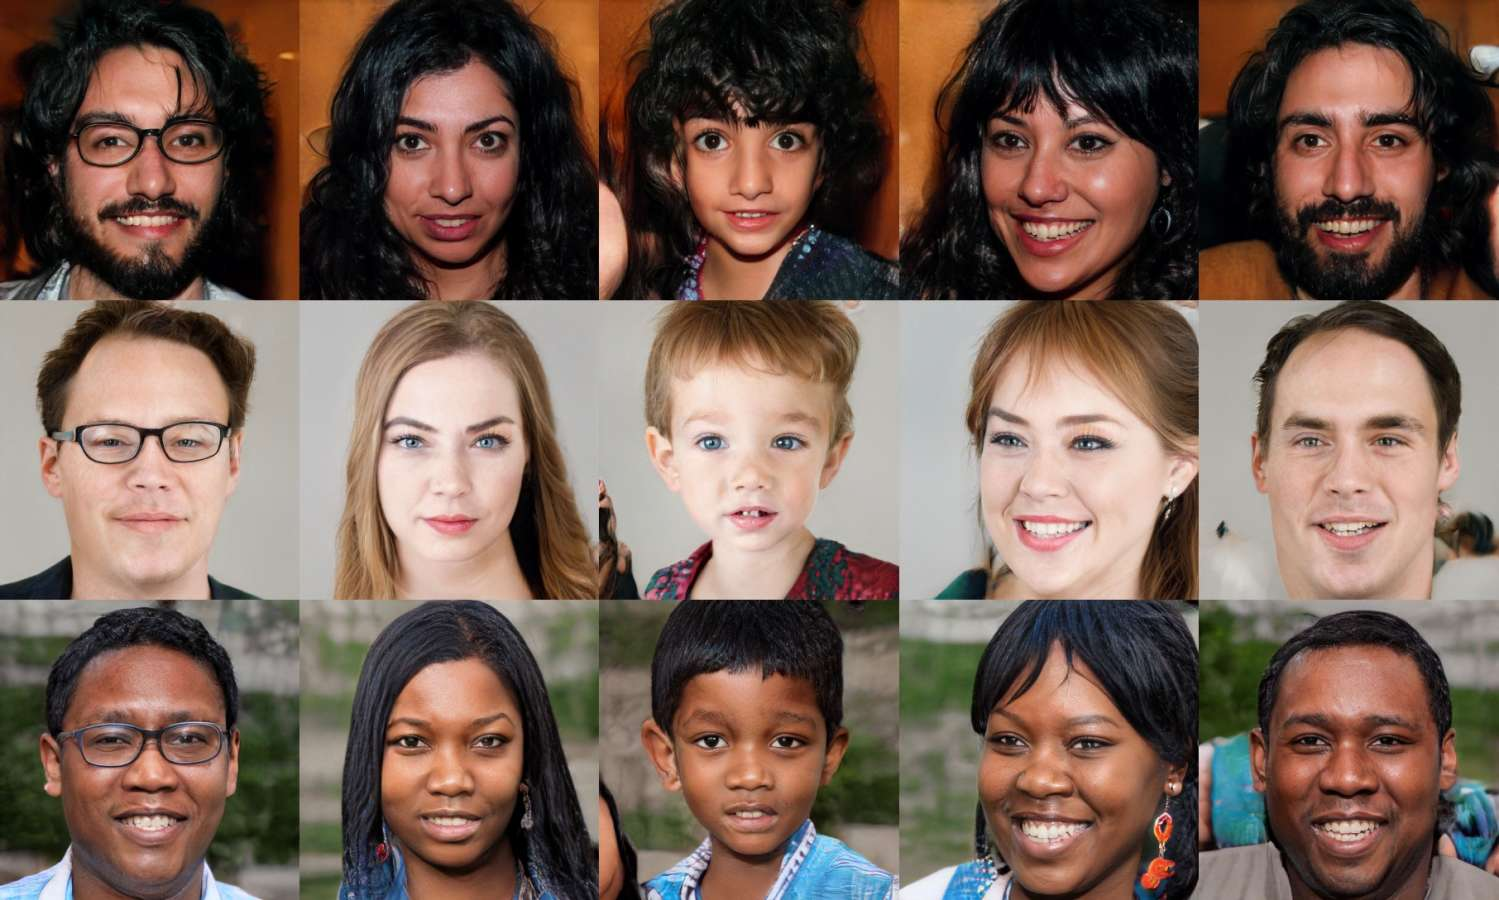
\includegraphics[width=0.6\textwidth]{imagenes/caras gan.png}
    \caption[Fotos de rostros humanos creados por una red GAN]{Fotos de rostros humanos creados por una red GAN. Tomado de \cite{Zavia2018}.}
    \label{fig:imagenes_gan}
\end{figure}

Realmente implementan una idea muy sencilla: pongamos a competir dos redes neuronales entre sí para que aprendan una de la otra indefinidamente. Una de ellas, llamada generador, generará una imagen falsa, mientras que la otra red, llamada discriminador, decide si la imagen es real o no. La figura \ref{fig:esquema_gan} muestra dicho esquema.

\begin{figure}[h]
    \centering
    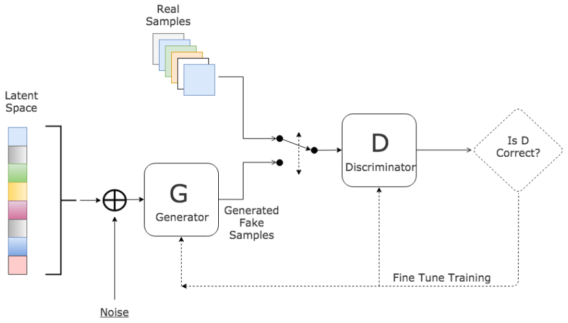
\includegraphics[width=1\textwidth]{imagenes/esquema gan.png}
    \caption[Esquema de una red GAN]{Esquema de una red GAN. Tomado de \cite{R.VIllatoro2018}.}
    \label{fig:esquema_gan}
\end{figure}

Esta competición tiene suma cero, es decir, el acierto de una de ellas se compensa con la pérdida de la opuesta, de forma que la que ha \textit{perdido} aprenda de ello. Eso nos permite refinar el modelo \textit{indefinidamente}, ya que ambas mejoran continuamente. Por ejemplo el generador aprenderá a generar imágenes más precisas, mientras el discriminador aprenderá cada vez mejor los rasgos de las fotos para evitar ser engañada.

\subsubsection{Generador: función y algoritmo de entreno}

El generador toma una distribución aleatoria como entrada (normalmente Gaussiana) y genera una imagen salida \cite{Geron2019}. Esta imagen comenzará siendo ruido aleatorio, para empezar a ofrecer resultados cada vez más realistas. \newline

Esta red se entrena después del discriminador y de forma totalmente diferente: el generador produce un conjunto exclusivo de imágenes falsas, las etiquetamos como imágenes reales y se las pasamos al discriminador (le intentamos engañar). El error cometido por el discriminador clasificando las imágenes falsas es el que usamos para entrenar el generador. Por ejemplo, si el discriminador ha etiquetado todas las imágenes como reales, entrenamos al generador con error 0 (es decir, no lo modificamos) puesto que le engaña perfectamente. En este paso los pesos del discriminador son congelados para que el entreno afecte únicamente al generador.

\subsubsection{Discriminador: función y algoritmo de entreno}

El generador únicamente se encarga de discernir si la imagen recibida es verdadera o falsa. Dicha imagen puede ser del conjunto de datos reales o del generador. \newline

El entreno de esta red se hace antes que el del discriminador, y se realiza como sigue: en primer lugar se compone un conjunto de imágenes para que las vea el generador: la mitad será del conjunto de imágenes real y la otra mitad del generador y a diferencia del caso anterior los etiquetamos como corresponde. Evaluamos los resultados, calculamos el error y el optimizador se encarga de modificar los pesos para la siguiente iteración. Es decir, su algoritmo de entrenamiento es el tradicional. Cabe decir que como en el caso del discriminador, los pesos de la otra red se congelan para que se entrene únicamente el generador.

\subsubsection{Las dificultades del entreno de las redes GAN}

Aunque a priori el juego de la competición entre redes puede dar muy buenos resultados, no los produce en todos los casos. Existe un estado final, llamado \textit{equilibrio de Nash} en el que ningún jugador mejora su comportamiento si cambia su estrategia si se asume que el rival no cambiará la suya. Por ejemplo, el equilibrio de Nash aparece en la vida real: los conductores circulan por el lado derecho de la calzada y ningún conductor \textit{mejora} por ir al lado izquierdo, pero también puede darse que los conductores aprendieran a conducir por el lado izquierdo y ninguno circulase de manera correcta \cite{Geron2019}. \newline

Para evitar los efectos adversos de este fenómeno los autores de las redes GAN demostraron que las redes GAN sólo producen un único equilbrio de Nash, y lo consiguen haciendo que las imágenes que recibe el discriminador en el entreno del generador sean 50\% reales y 50\% falsas. Por otra parte esto no garantiza que la red alcance este equilibrio, además de que incrementa el tiempo de entrenamiento. \newline

No es la única dificultad que tienen: su mayor problema es el denominado \textit{modo colapso} o \textit{mode collapse} en inglés: se produce cuando el generador va perdiendo diversidad en sus salidas, perdiendo gradualmente toda su \textit{creatividad}. \newline

Para explicar este fenómeno utilizaré el ejemplo presentado en \cite{Geron2019}: supongamos que tenemos un conjunto de datos que sean prendas de ropa y el generador produzca mucho mejor zapatos que otra cosa. Como engaña mejor al discriminador que produciendo otra cosa, el generador comenzará a generar cada vez más zapatos, olvidando cómo se generan otras prendas de ropa. Lo mismo le pasará al discriminador: se centrará tanto en describir zapatos que olvidará cómo son las otras prendas. Llegará un momento en el que el discriminador sepa perfectamente cómo distinguir los zapatos reales de los falsos, por los que el generador buscará otra prenda de ropa (por ejemplo camisetas), olvidando gradualmente cómo eran los zapatos y así sucesivamente. \newline

Esto provoca que a veces la red GAN no converja o que su entrenamiento sea muy inestable. Como esto se produce por numerosos factores, las redes GAN sean muy sensibles a los hiperparámetros (el conjunto de parámetros fijado por el programador). \newline

Por tanto, vemos que las redes GAN presentan una serie de problemas, si bien los investigadores están proponiendo nuevas técnicas para solucionarlas. Como esas soluciones son dependientes del problema y no son necesarias para entender las redes GAN, no las incluimos en este documento.


\subsection{Transferencia de estilo y Cycle GAN}
\subsubsection{Transferencia de estilo}

La transferencia de estilo es el concepto que queremos implementar en este \tfg, ya que el concepto designa a un sistema que es capaz de transformar una imagen de entrada a otro dominio diferente \cite{Foster2019}. Aquí toca realizar una matización: el objetivo de este \tfg es emular el estilo propio de un pintor, no de un sólo cuadro del pintor. \newline

Esta técnica nos permite cambiar el dominio por otro cualquiera, por lo que el sistema es válido para otro pintor, únicamente cambia el entrenamiento del mismo. Esto permite a que el lector pueda implementar sus propios modelos a partir de sus propias imágenes u obteniendo los cuadros de otros pintores. \newline

Las dos técnicas más populares dentro del campo de la transferencia de estilo son las Redes Generativas Antagónicas Cíclicas y la Transferencia de Estilo Neuronal. \newline

La primera de ellas es la que implementaremos en este \tfg, ya que el conjunto de destino puede tener un número arbritario de fotos y permite que el sistema aprenda el estilo del pintor; mientras que la Transferencia de Estilo Neuronal (\textit{Neural Style Transfer} en inglés) únicamente permite el aprendizaje de una sola obra.  \newline

La figura \ref{fig:chibi_jl} muestra un montaje realizado y cedido por Juan Luis Moreno Sancho, amigo del autor, realizado mediante \textit{Neural Style Transfer}. \newline

\begin{figure}[h]
    \centering
    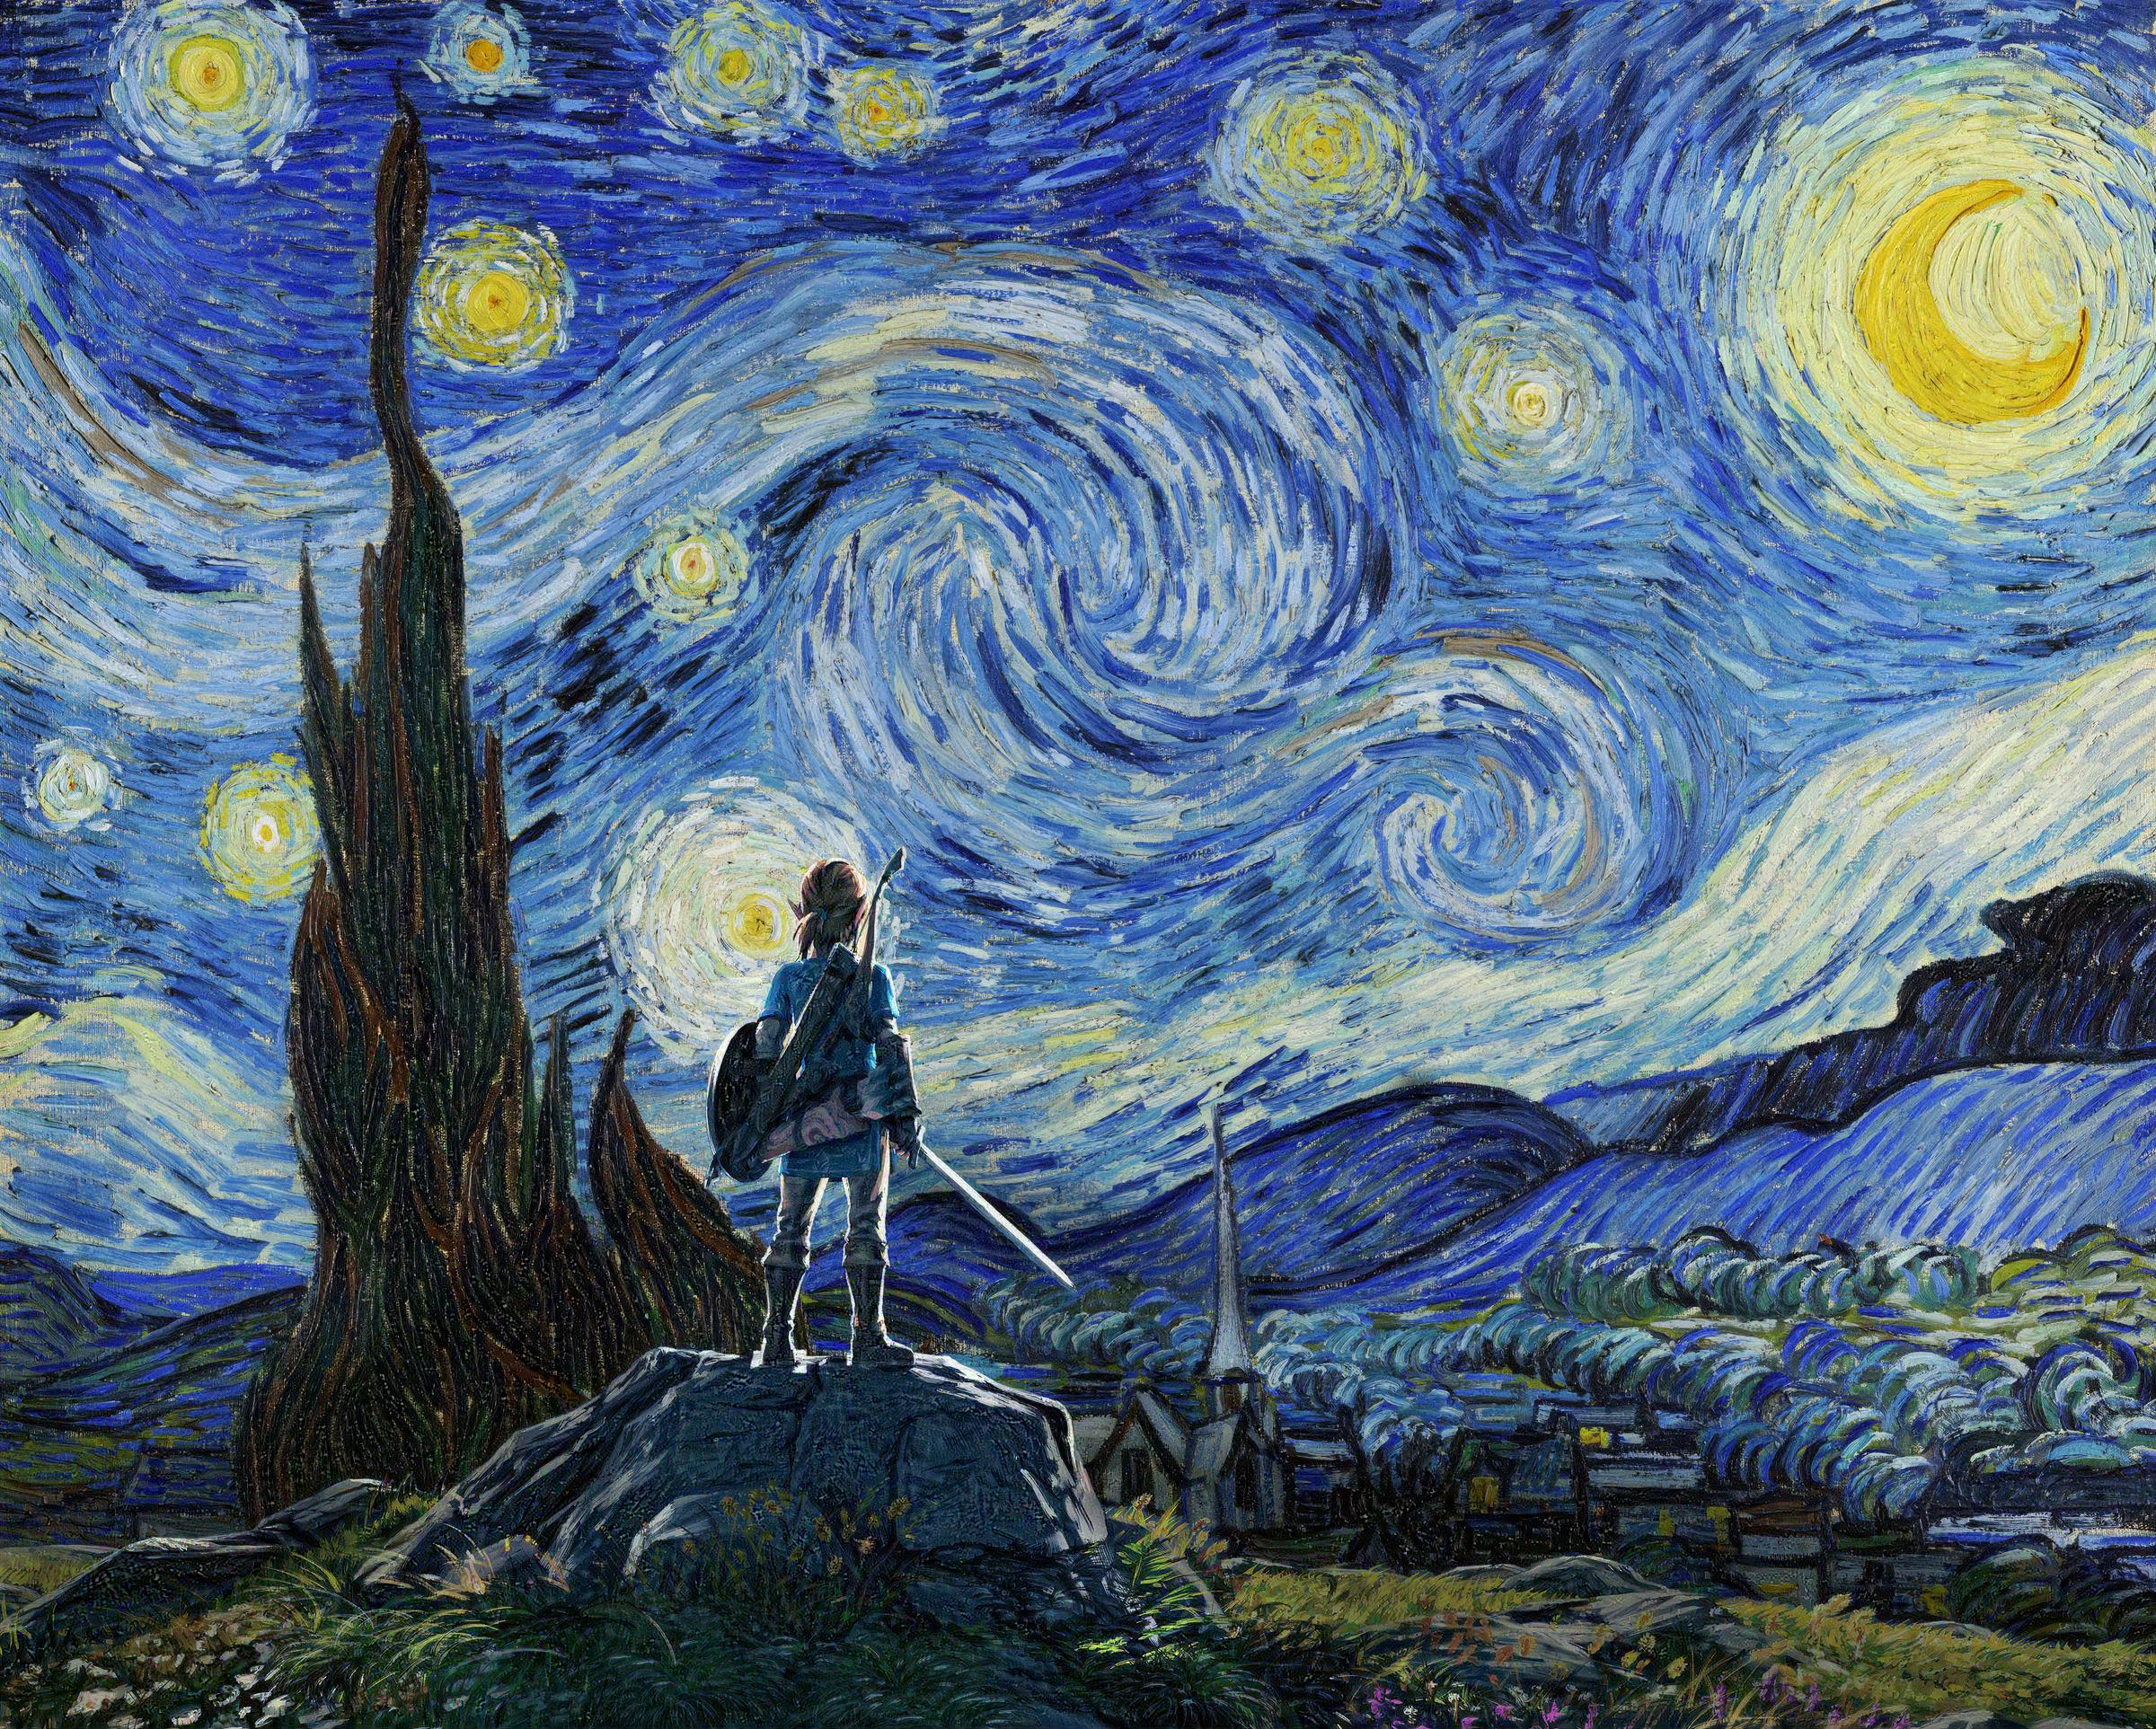
\includegraphics[width=0.6\textwidth]{imagenes/chibi_jl.jpg}
    \caption[Montaje de Zelda y La noche estrellada]{Montaje de Zelda y La noche estrellada. Obra de Juan Luis Moreno Sancho.}
    \label{fig:chibi_jl}
\end{figure}

\subsubsection{Cycle GAN}
\label{Cycle GAN}

Las Redes Generativas Antagónicas Cíclicas, conocidas como \textit{Cycle GAN}, es una red que consiste en dos redes GAN intercomunicadas entre sí \cite{Zhu2017}. Este sistema permite la implantación de nuestro objetivo principal: la conversión de fotos a cuadros, pero \textit{Cycle GAN} es más que eso: permite convertir los dos dominios de forma bidireccional, lo que nos permite pasar de fotos a cuadros y de cuadros a fotos (es decir, el paisaje que trataron de \textit{imitar} los pintores). \newline

Además de la bidireccionalidad de las conversiones, su mayor ventaja frente a otros modelos como \textit{pix2pix} es que no se necesitan pares de ejemplos \footnote{Por pares de ejemplos nos referimos a disponer del mismo elemento en ambos dominios. Un par podría ser las palabras \textit{hola} en castellano y \textit{hello} en inglés}. Esa característica es la que hace posible que nuestro objetivo pueda implementarse, ya que no disponemos, por ejemplo, de los paisajes que veía Monet en sus cuadros. \newline

Por último, una \textit{Cycle GAN} son dos redes GAN unidas entre sí. Por tanto tenemos dos generadores y dos discriminadores. Uno de los generadores pasa del dominio del pintor al fotográfico, mientras que el otro hace la transformación inversa. Al no tener pares de ejemplos para entrenar nuestros generadores, tenemos que entrenar los dos discriminadores para ver si las imágenes son válidas o no, tal y como hacíamos en una red GAN cualquiera. Por tanto, tenemos un discriminador que será capaz de distinguir fotografías de falsificaciones, y otro que hará lo mismo pero con los cuadros. \cite{Foster2019} \newline

\begin{figure}[h]
    \centering
    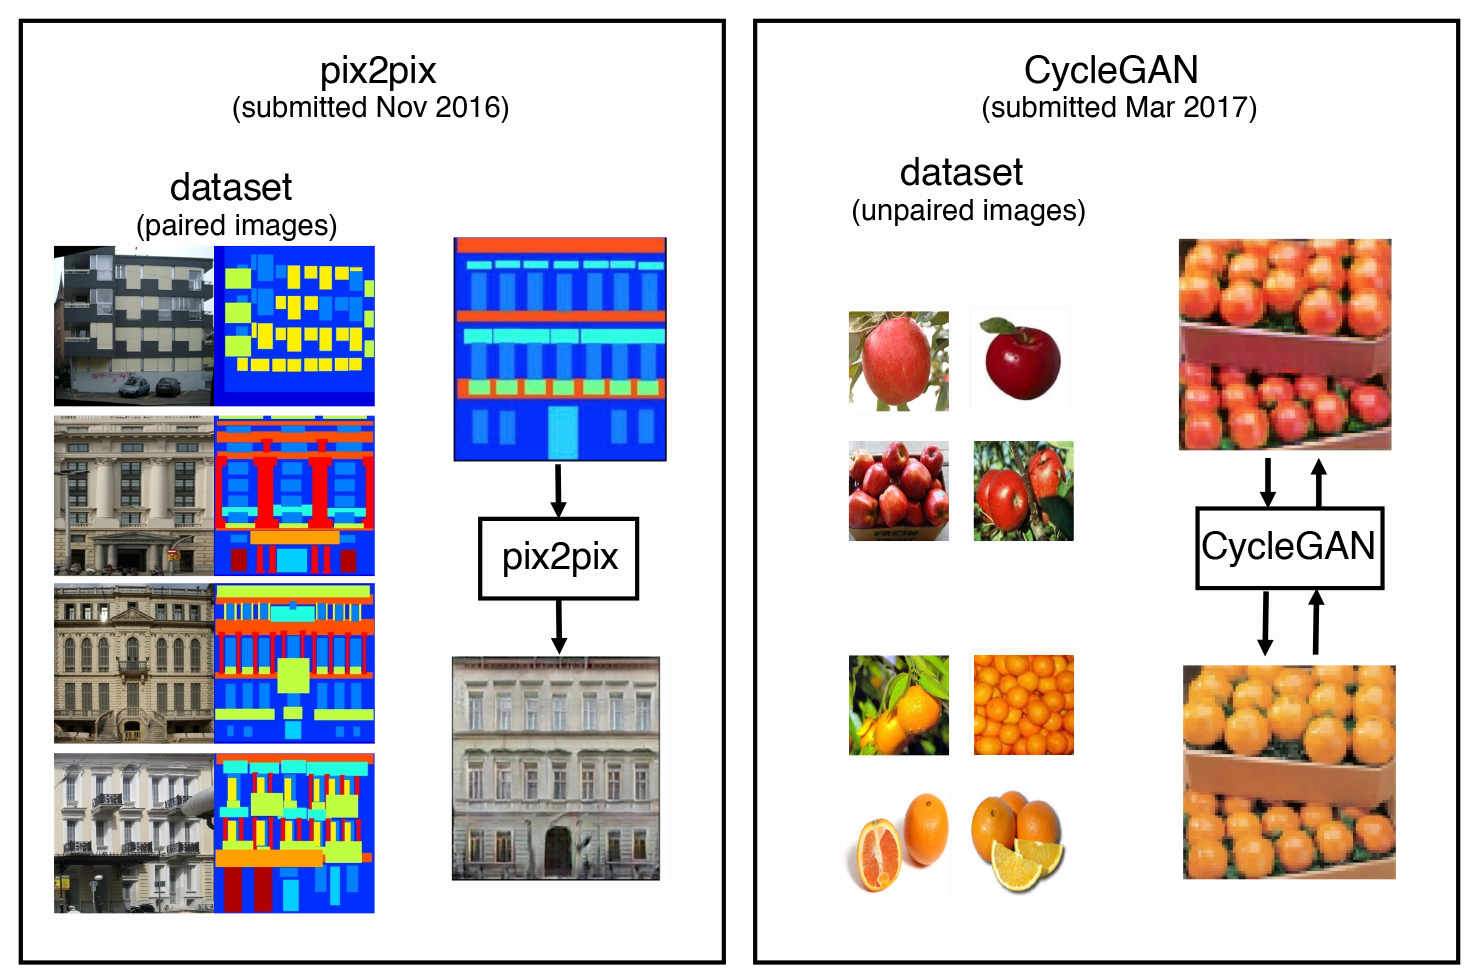
\includegraphics[width=0.66\textwidth]{imagenes/pix2pix y cyclegan.png}
    \caption[Comparativa entre pix2pix y Cycle GAN]{Comparativa entre pix2pix y Cycle GAN. Extraido de \cite{Foster2019}}
    \label{fig:pix2pixVScycleGAN}
\end{figure}
\newpage
\end{document}